%%%%%%%%%%%%%%%%%%%%%%%%%%%%%%%%%%%%%%%%%%%%%%%%%%%%%%%%%%%%%%%%%%% 
%                                                                 %
%                            CHAPTER                              %
%                                                                 %
%%%%%%%%%%%%%%%%%%%%%%%%%%%%%%%%%%%%%%%%%%%%%%%%%%%%%%%%%%%%%%%%%%% 
 
\chapter{Implementation}


\section{Camera setup}
Carbide tool inserts are not yet items that are much researched so there are no big datasets that can be used to train and test algorithms on. Therefore a new dataset must be created with worn tool inserts. For the creation of the dataset a setup is created. This setup consists of three different parts:
\begin{enumerate}
\item A tool holder which will provide the same position for the tool for every picture
\item A mount for the microscopic camera which is easy to finetune
\item Some lighting solution that provides the right angle of light to the tool insert.
\end{enumerate}

	\subsection{Design of a tool holder}
	The tool holder will be the most important part of the setup since this part will be holding the tool insert. The requirements for this holder are that the tool is easily removable to replace inserts. It may not be visible to the camera or provide very small mounts of distraction or occlusion.
	
	
	\subsubsection{First tool holder}
	All tool holder prototypes where 3D printed. A first holder was made to check how the lighting would be transferred to the camera. This was put in a simple setup with a desk lamp, a holder which kept the insert at an angle of 40\textdegree. This showed potential in the current setup as seen in Figure \ref{fig:impl:setup:deskholder}. The tool wear is nicely indicated with the reflections of the light. 
	
	\begin{figure}[hbtp]
	\centering
	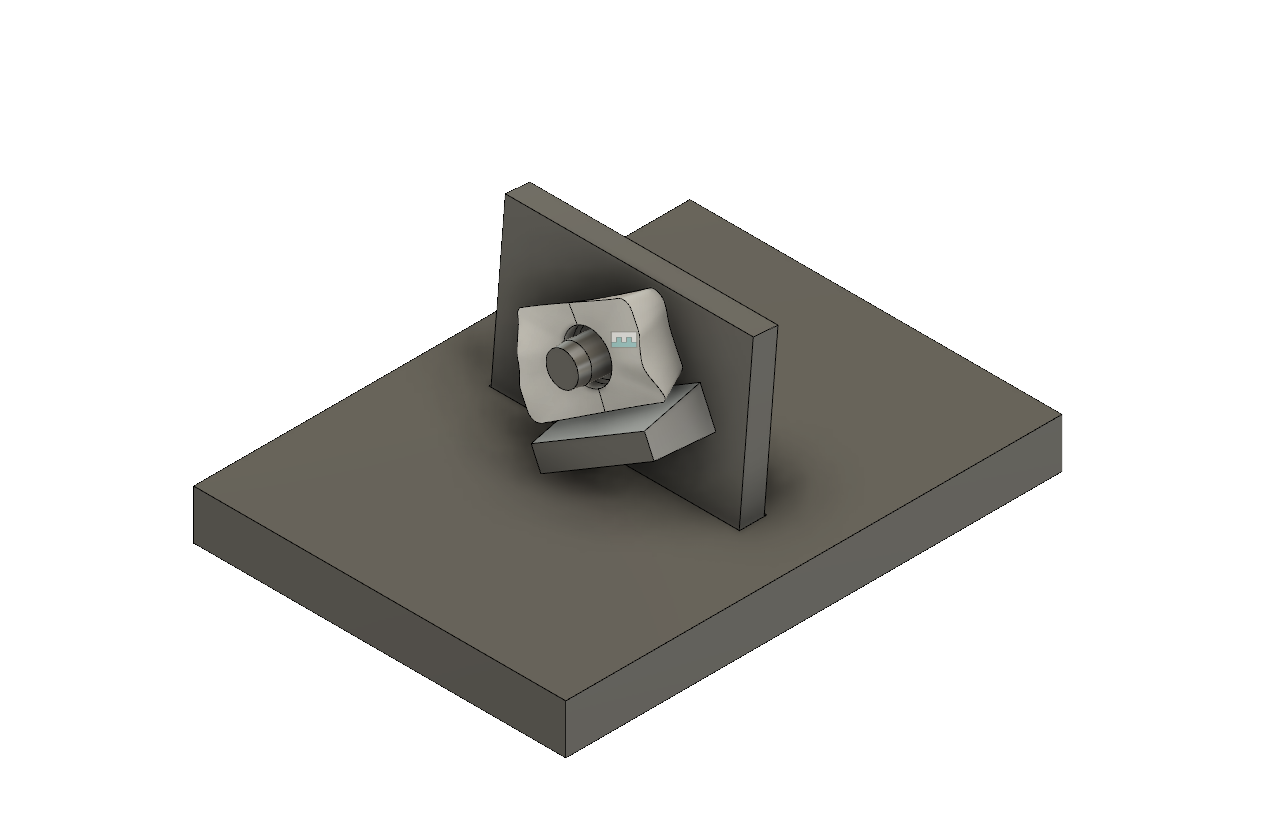
\includegraphics[scale=0.2]{fig/Camera_setup/Tool_Holder/simpeleHouder_attaached.png}
	\caption{First design of a tool holder oriented at an angle of 40\textdegree to the camera.}
	\end{figure}
	

	\subsubsection{Wheel holder}
	The previous first tool holder was good for taking a sample picture of an image but isn't scalable to take pictures of a few hundreds of inserts.
	To be able to quickly create a lot of photos in a consistant way, a wheel is designed to mount 20 tools at once using a stepper motor and a fixed camera and lighting setup. The process of taking images would be automated for every 20 tools. The holder is 3D printed so a few wheels can be made to be able to swap the wheels with new tools for an efficient dataset creation.
	
		The first test of this wheel holder can be seen in Figure \ref{fig:setup:wheelholder1:inserts}. Here everything is printed in one piece. The inserts are kept in place with brackets that go over the cutting edge of the insert. This wasn't ideal since the sharp edges of the insert would clamp in the bracket what made it very hard to remove the tools and didn't comply with the easy removal constraint. 
		
		
		\begin{figure}[hbtp]
		\centering
		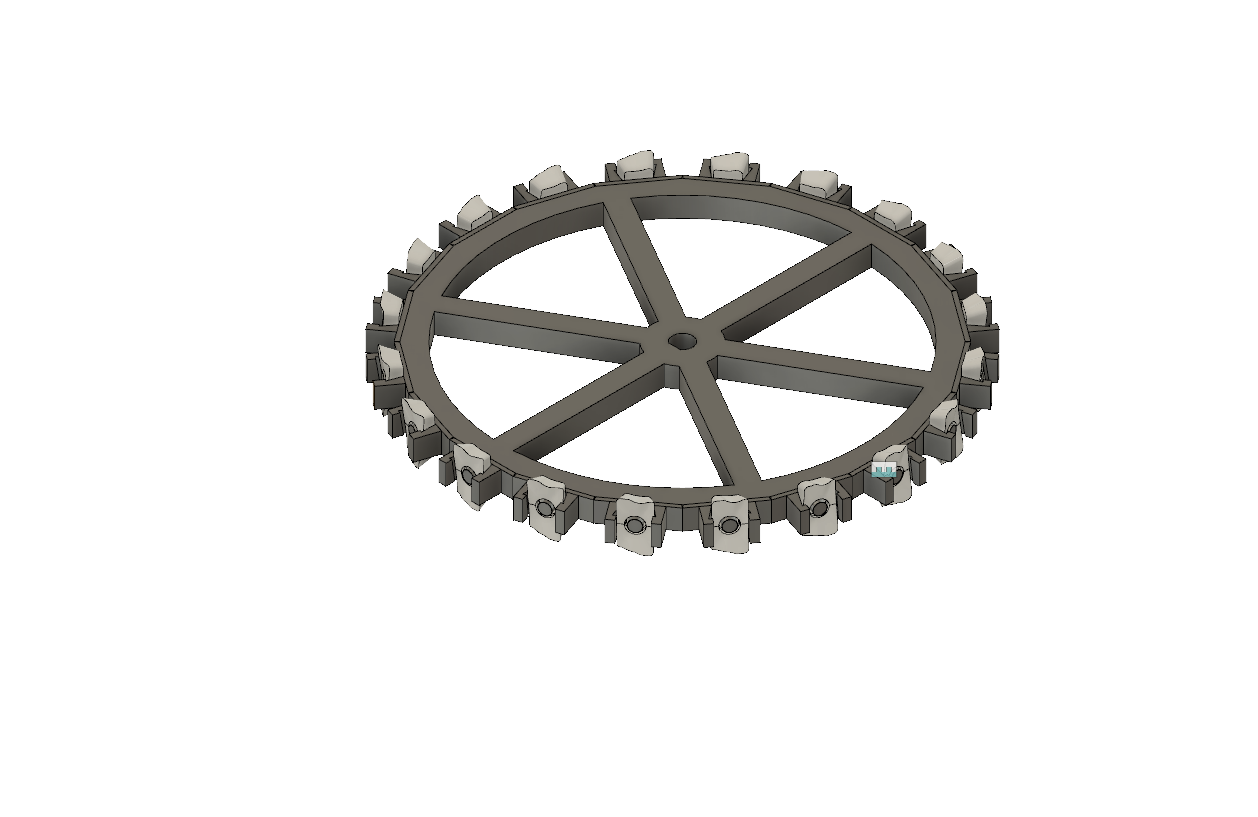
\includegraphics[scale=0.3]{fig/Camera_setup/Tool_Holder/Wheel_Holder/first_wheel_holder/radhouderV1_model_inserts.png}
		\caption{First design of wheel holder with inserts mounted in place.}
		\label{fig:setup:wheelholder1:inserts}
		\end{figure}
		
		For this reason a second wheel was designed which was a little more flexible and made the process of inserting and replacing tools a lot easier by providing a clip which was printed and added to the insert separately. Figure \ref{fig:setup:wheelholder2:inserts} shows the full assembly of this second wheel holder. 
		
		
		\begin{figure}[hbtp]
		\centering
		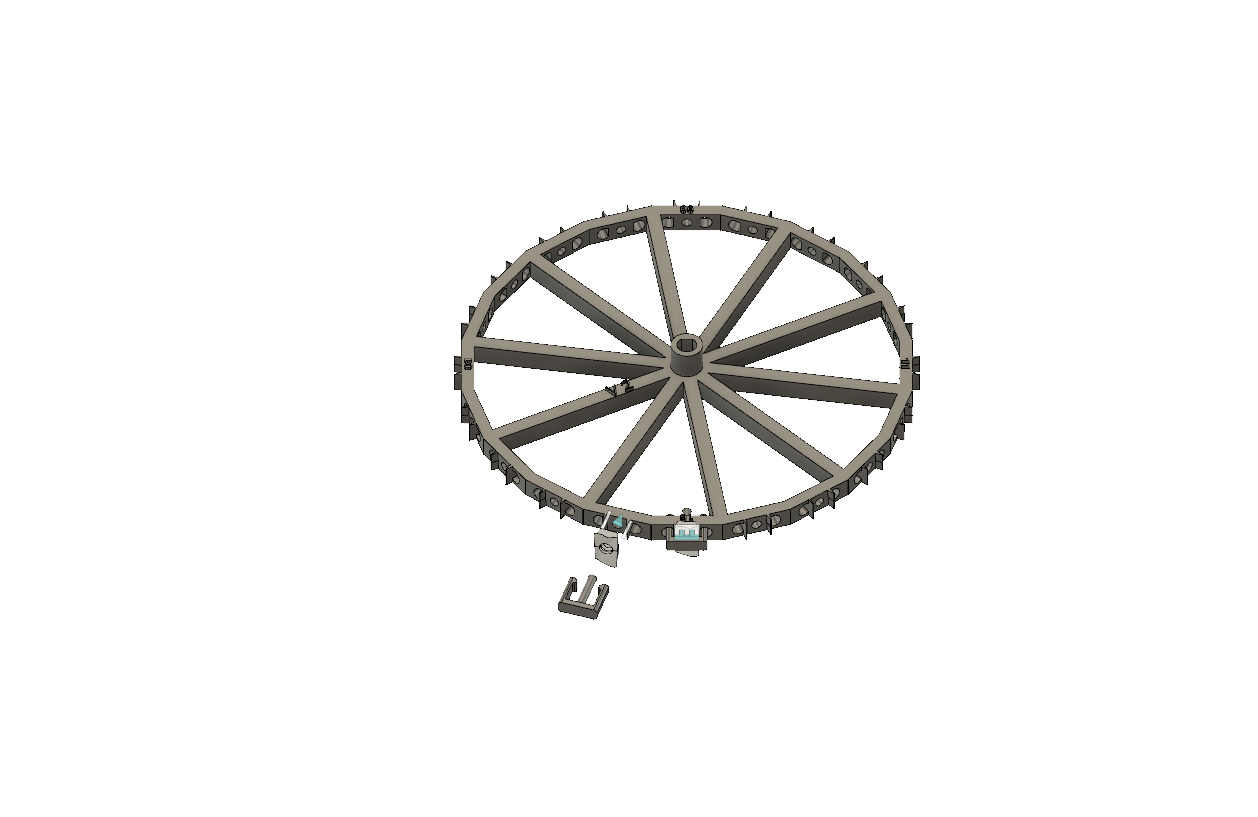
\includegraphics[scale=0.3]{fig/Camera_setup/Tool_Holder/Wheel_Holder/Second_Wheel_Holder/radhouder_v2_assembly.png}
		\caption{Second wheel holder with clip and insert.}
		\label{fig:setup:wheelholder2:inserts}
		\end{figure}
		
		In the wheel there are holes in which the clips fit. The center hole is as big as the hole in the inserts. This keeps the insert from moving when the clip is on. The slads between the holes are made to fit the insert perfectly so this doesn't rotate around the axis of the clip. On the clip there is an extra long middle tube that makes it easier to push the clip with the insert out of the wheel.

The printing of these wheels was very difficult since it was with another material as we were used to and the print wouldn't stick to the print bed. This made a few bad runs and hours of wasted printing time. At the end 8 wheels of this are printed correctly and were used to create the datasets.
		
	\subsection{Design of a camera mount}
	In this page the camera mount will be discussed along the design process of the setup
		Since the camera mount provided by the factory was not up to the task of taking consistent pictures and controlling the camera position precisely, a new camera mount was designed. For this task some 20mm by 20mm aluminium profiles where used as a base for the stand. On that stand an assembly of 3D printed parts where mounted to be able to rotate the camera around two different axis. 
		
		insert assembly of full camera mount
		
	\subsection{Light configuration}
	In order to test different lighting options there must be a simple to configure lighting solution. Which is configurable in both color and light direction to create a maximum reflection of the wear area into the camera lens. This is achieved with single led adressable light.
	
	Multiple different light sources where tested as listed underneath. Some worth noticing are declared after.

		\begin{enumerate}
			\item Warm white led desk Lamp
			\item Long hard white led strips 
			\item single led adressable RGB led strip
			\item Multiple single led adressable RGB strips
			\item USB microscope camera light
		\end{enumerate}
		
		\subsubsection{Desk Lamp Test}

As an initial setup to test the camera and be able to see the effects of lighting on the image this setup was created and a desk lamp was used for the lighting as seen in Figure \ref{fig:setup:desklamp}.

\begin{figure}[hbtp]
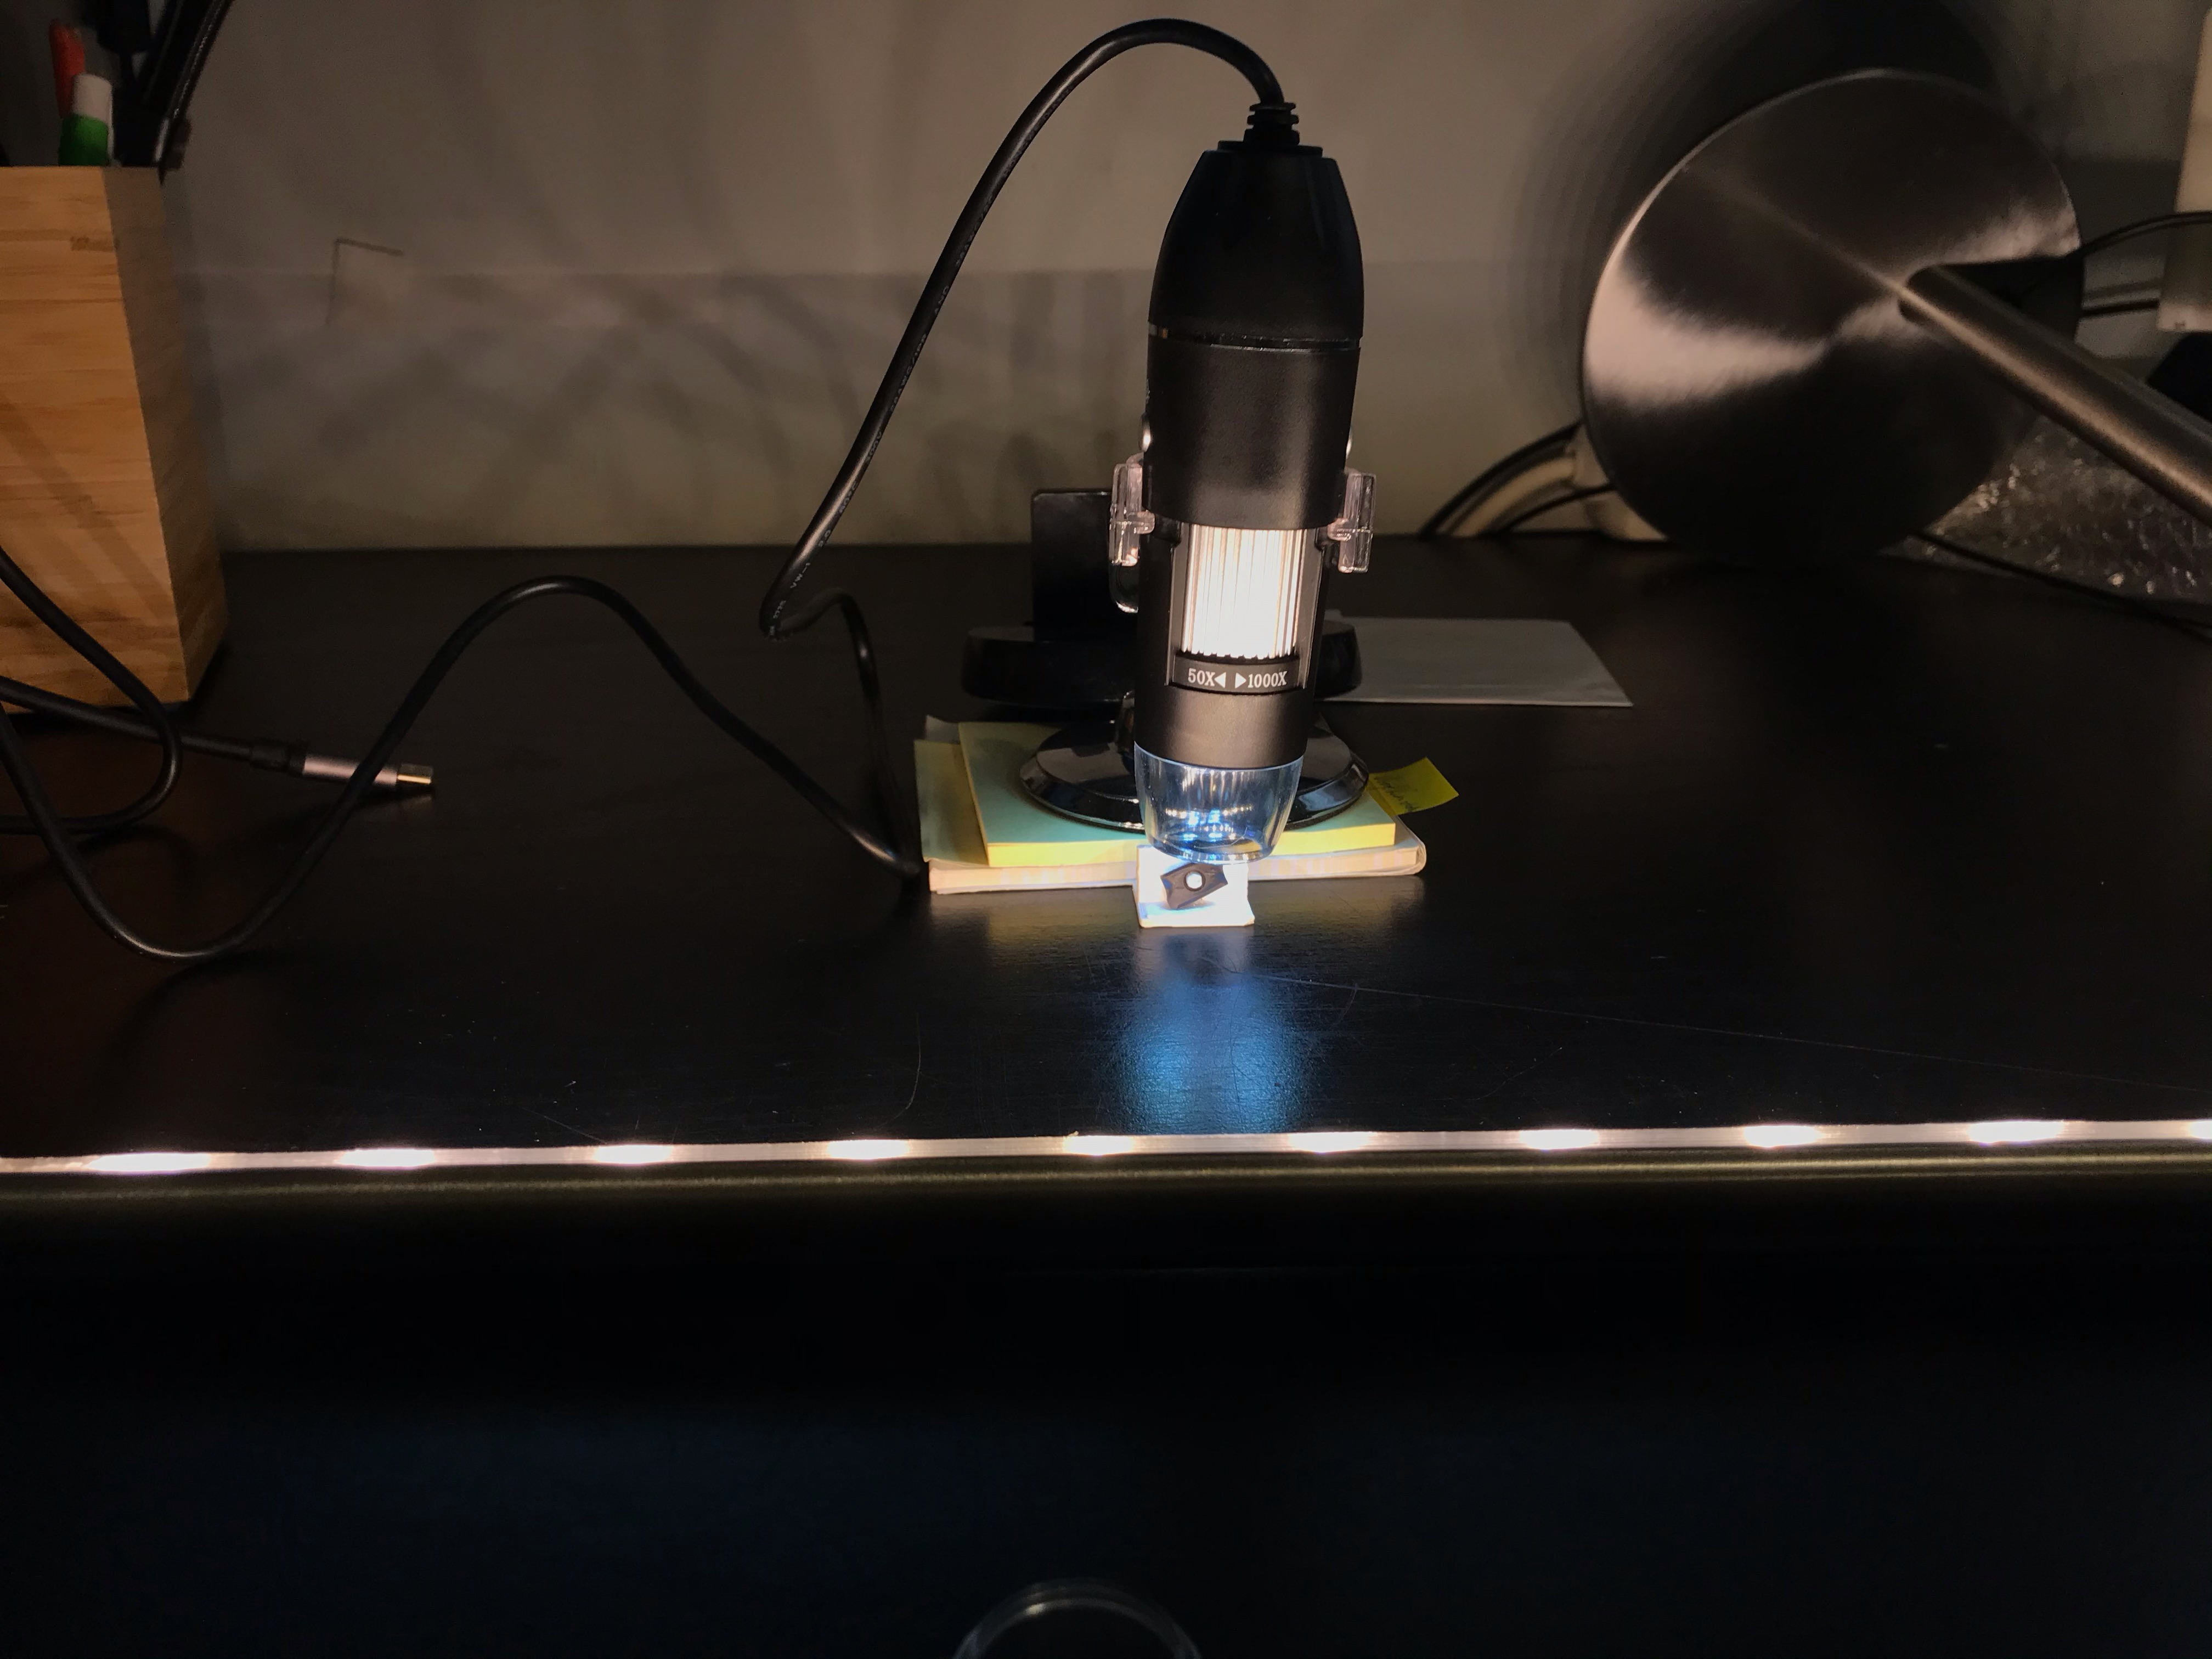
\includegraphics[width=4.166667in, keepaspectratio=true]{./fig/Camera_setup/Light/Desk_Lamp_Test/eerste_setup_andere_richting.jpeg}
\caption{Desk lamp setup for initial testing.}
\label{fig:setup:desklamp}
\end{figure}

This setup was using the top light of the camera. This light was good to be able to adjust the camera. Without the light, the errornous places where more visible. But the desk lamp had to much brightness and didn't leave enough room for adjusting different settings. For this reason other lighting options where explored.

From this setup it can also be seen that the lighting on the background is important. Figure \ref{fig:setup:desklamp:whitebg} shows a picture of the tool with desk lamp lighting without blocking the light from the areas where it shouldn't be. Here we can see that there is a bright white background behind the tool. 

\begin{figure}[hbtp]
\centering
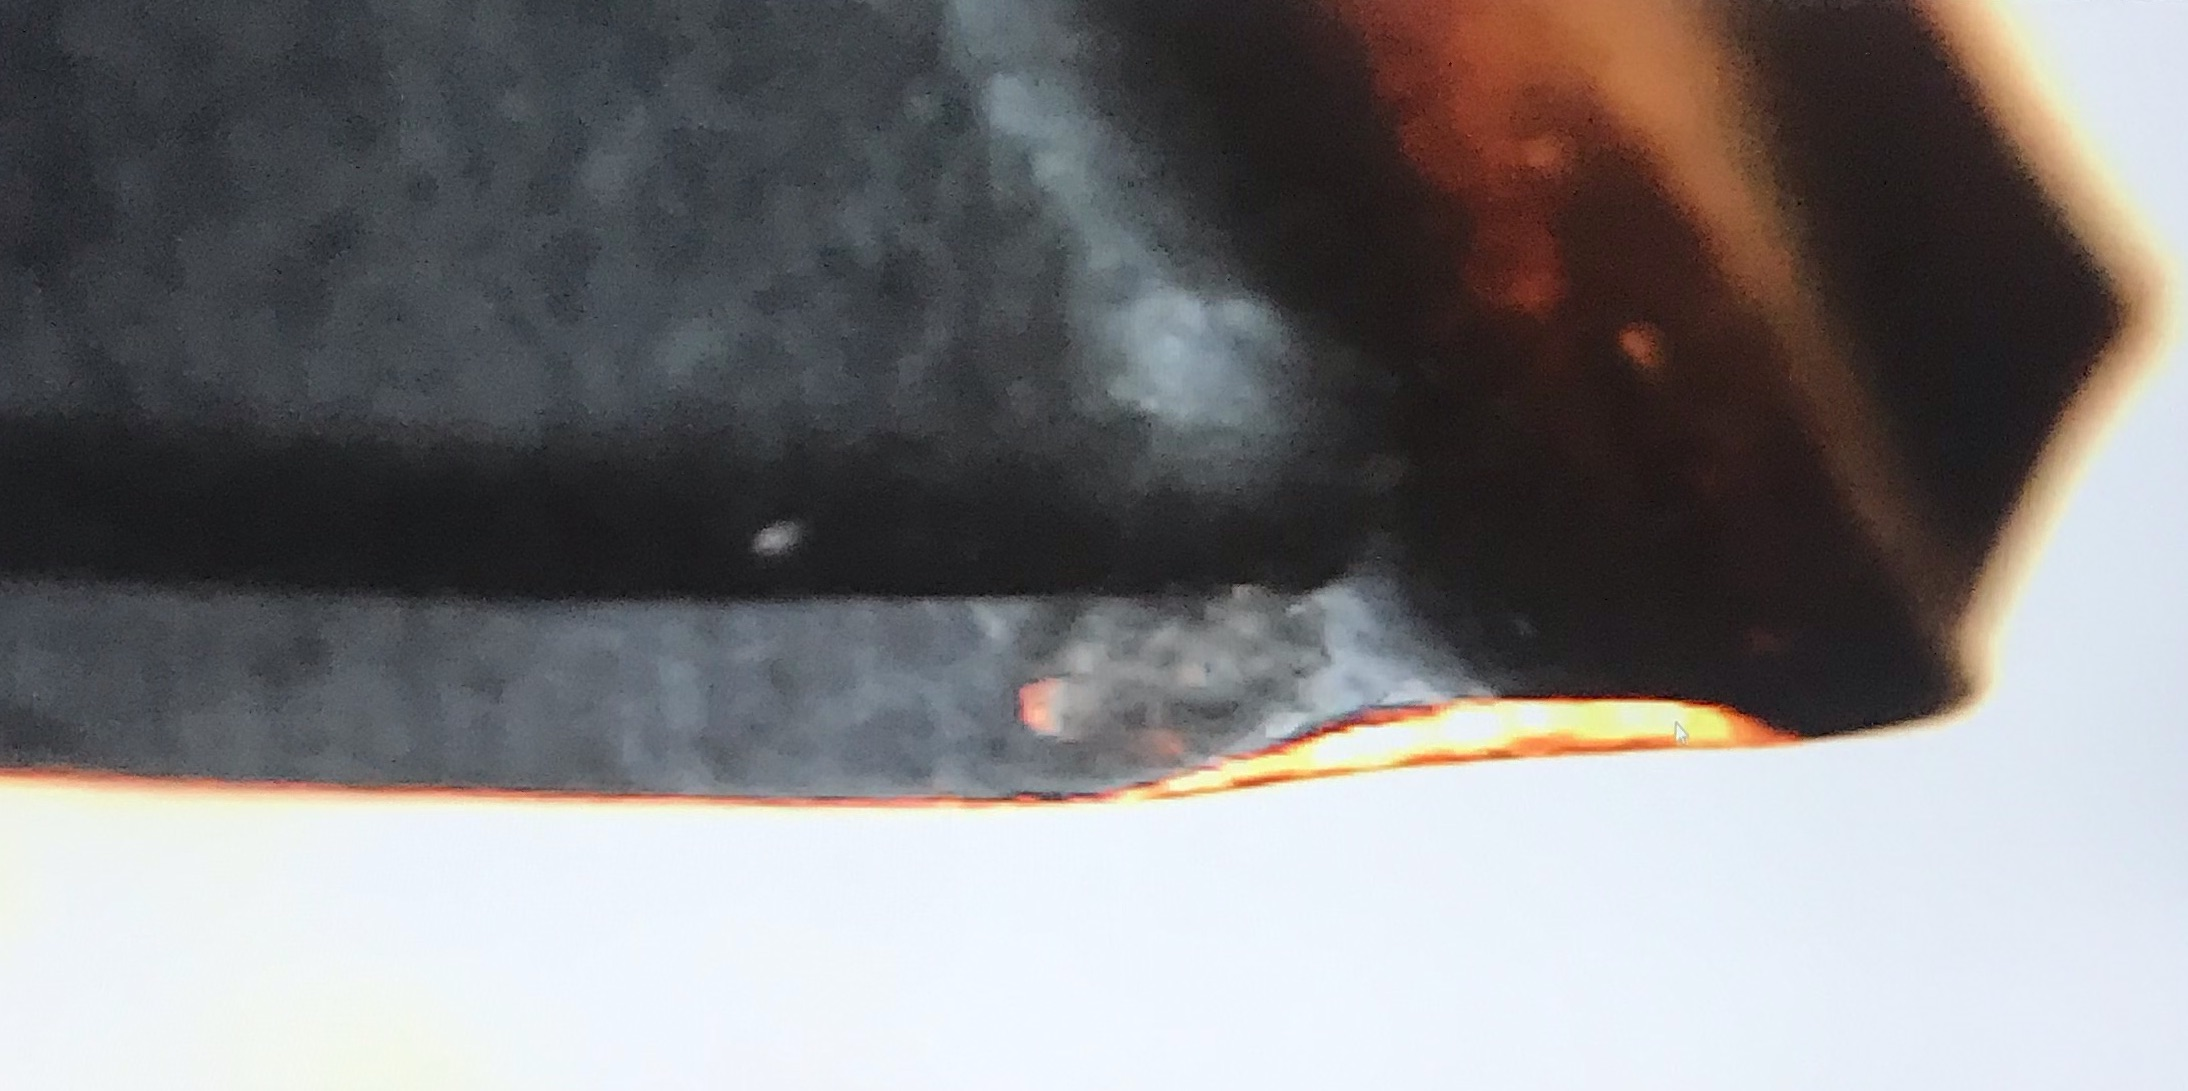
\includegraphics[scale=0.2]{fig/Camera_setup/Light/Desk_Lamp_Test/desk_lamp_setup_whitebg.jpeg}
\caption{Desk lamp setup without shadowing the background.}
\label{fig:setup:desklamp:whitebg}
\end{figure}


The result of this is shown in Figure \ref{fig:setup:desklamp:blackbg} where the light is blocked off of the rest of the tool and only the errornous part is lightened. This would be a good start to start creating a dataset.

\begin{figure}[hbtp]
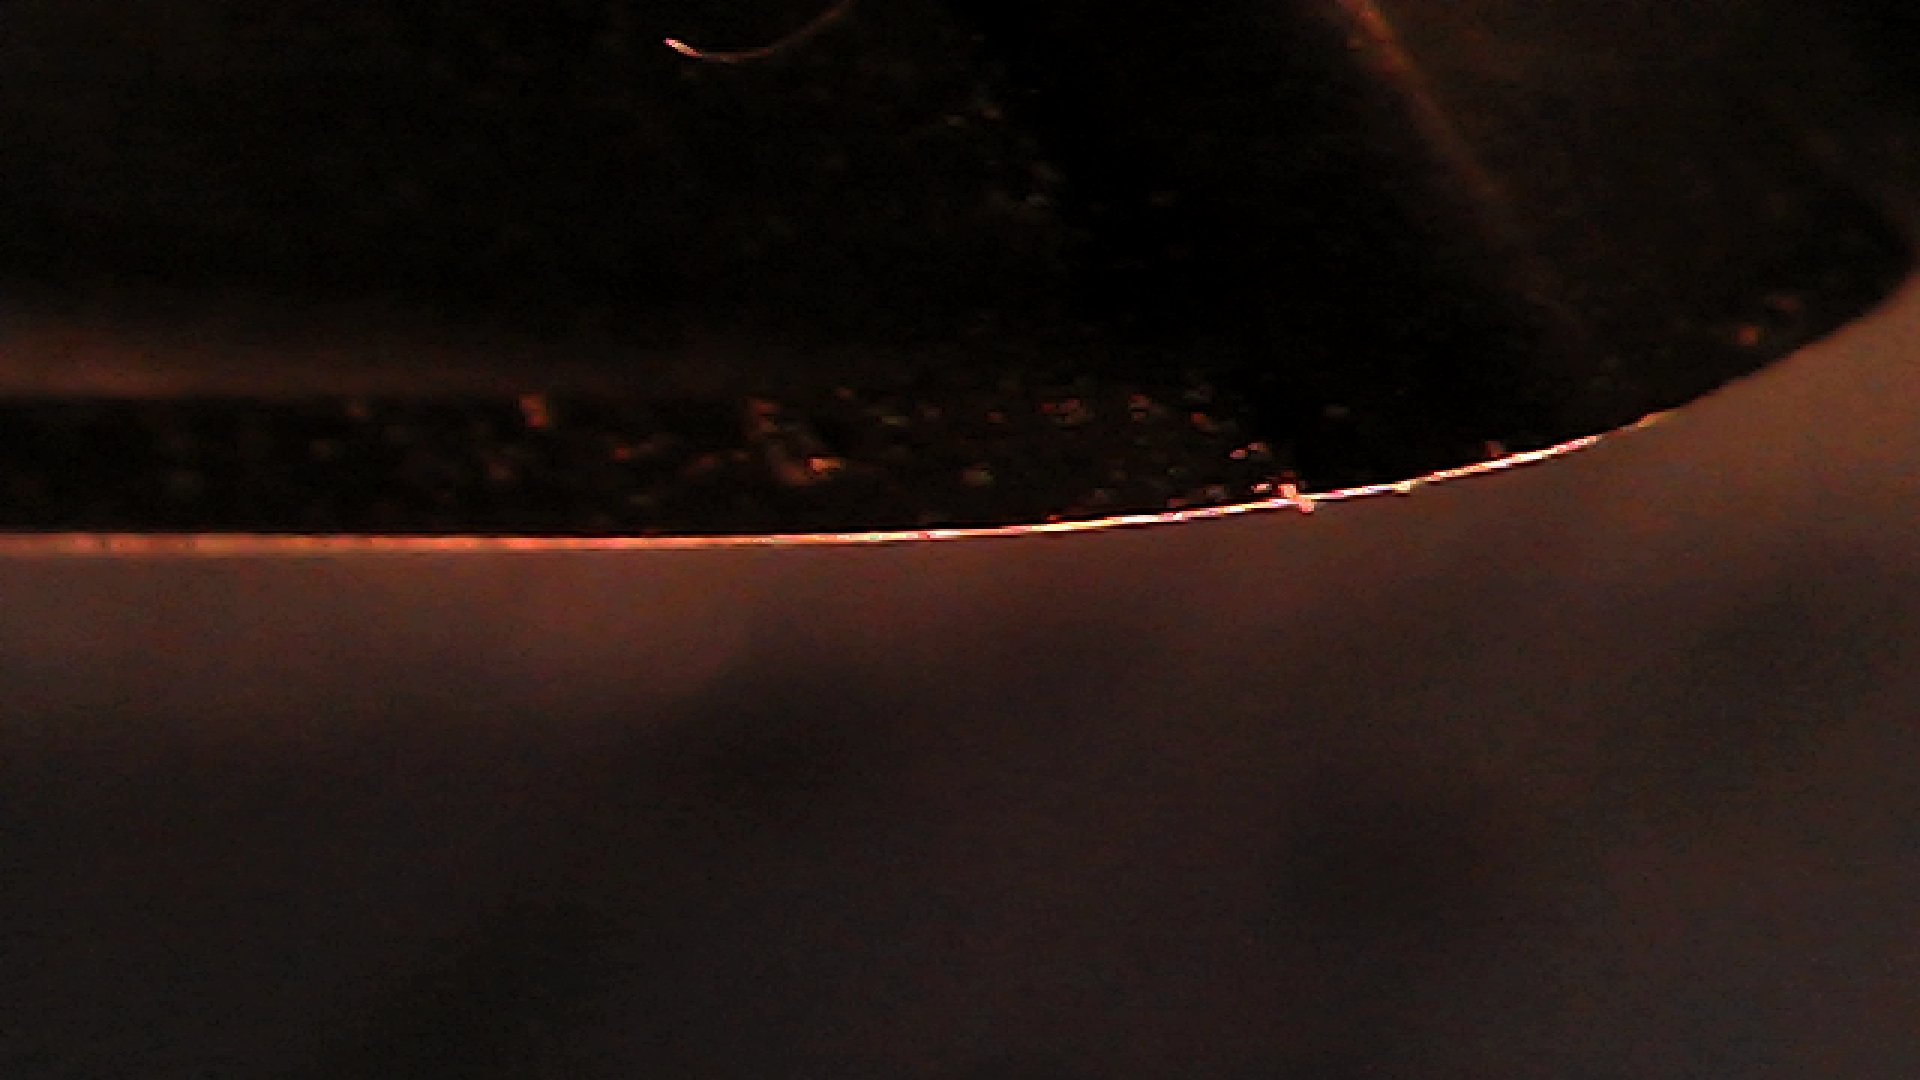
\includegraphics[width=4.166667in, keepaspectratio=true]{./fig/Camera_setup/Light/Desk_Lamp_Test/eerste-opstelling_donkere_achtergrond2.jpg}
\caption{Desk lamp setup with shadowing the background.}
\label{fig:setup:desklamp:blackbg}
\end{figure}

The color of the desk light set a good gradient of bad vs good sets. White areas are worn very hard while orange is not worn that hard.By tilting the lamp up and down in a horizontal way, all the areas where ligthtend. 


		\subsubsection{White Led Strips}

		A second lighting contition created is the lighting with 3 the same led strips controllable with a raspberry pi. 
		For the purpose of this test a small electric circuit is created to control these strips since they use more power than the raspberry pi can deliver \cite{rpi}. An overview of the test circuit can be found in Figure \ref{fig:setup:whiteled:circuit}. A potentiometer was used to control the voltage over the led strip in order to control the brightness. 


\begin{figure}[hbtp]
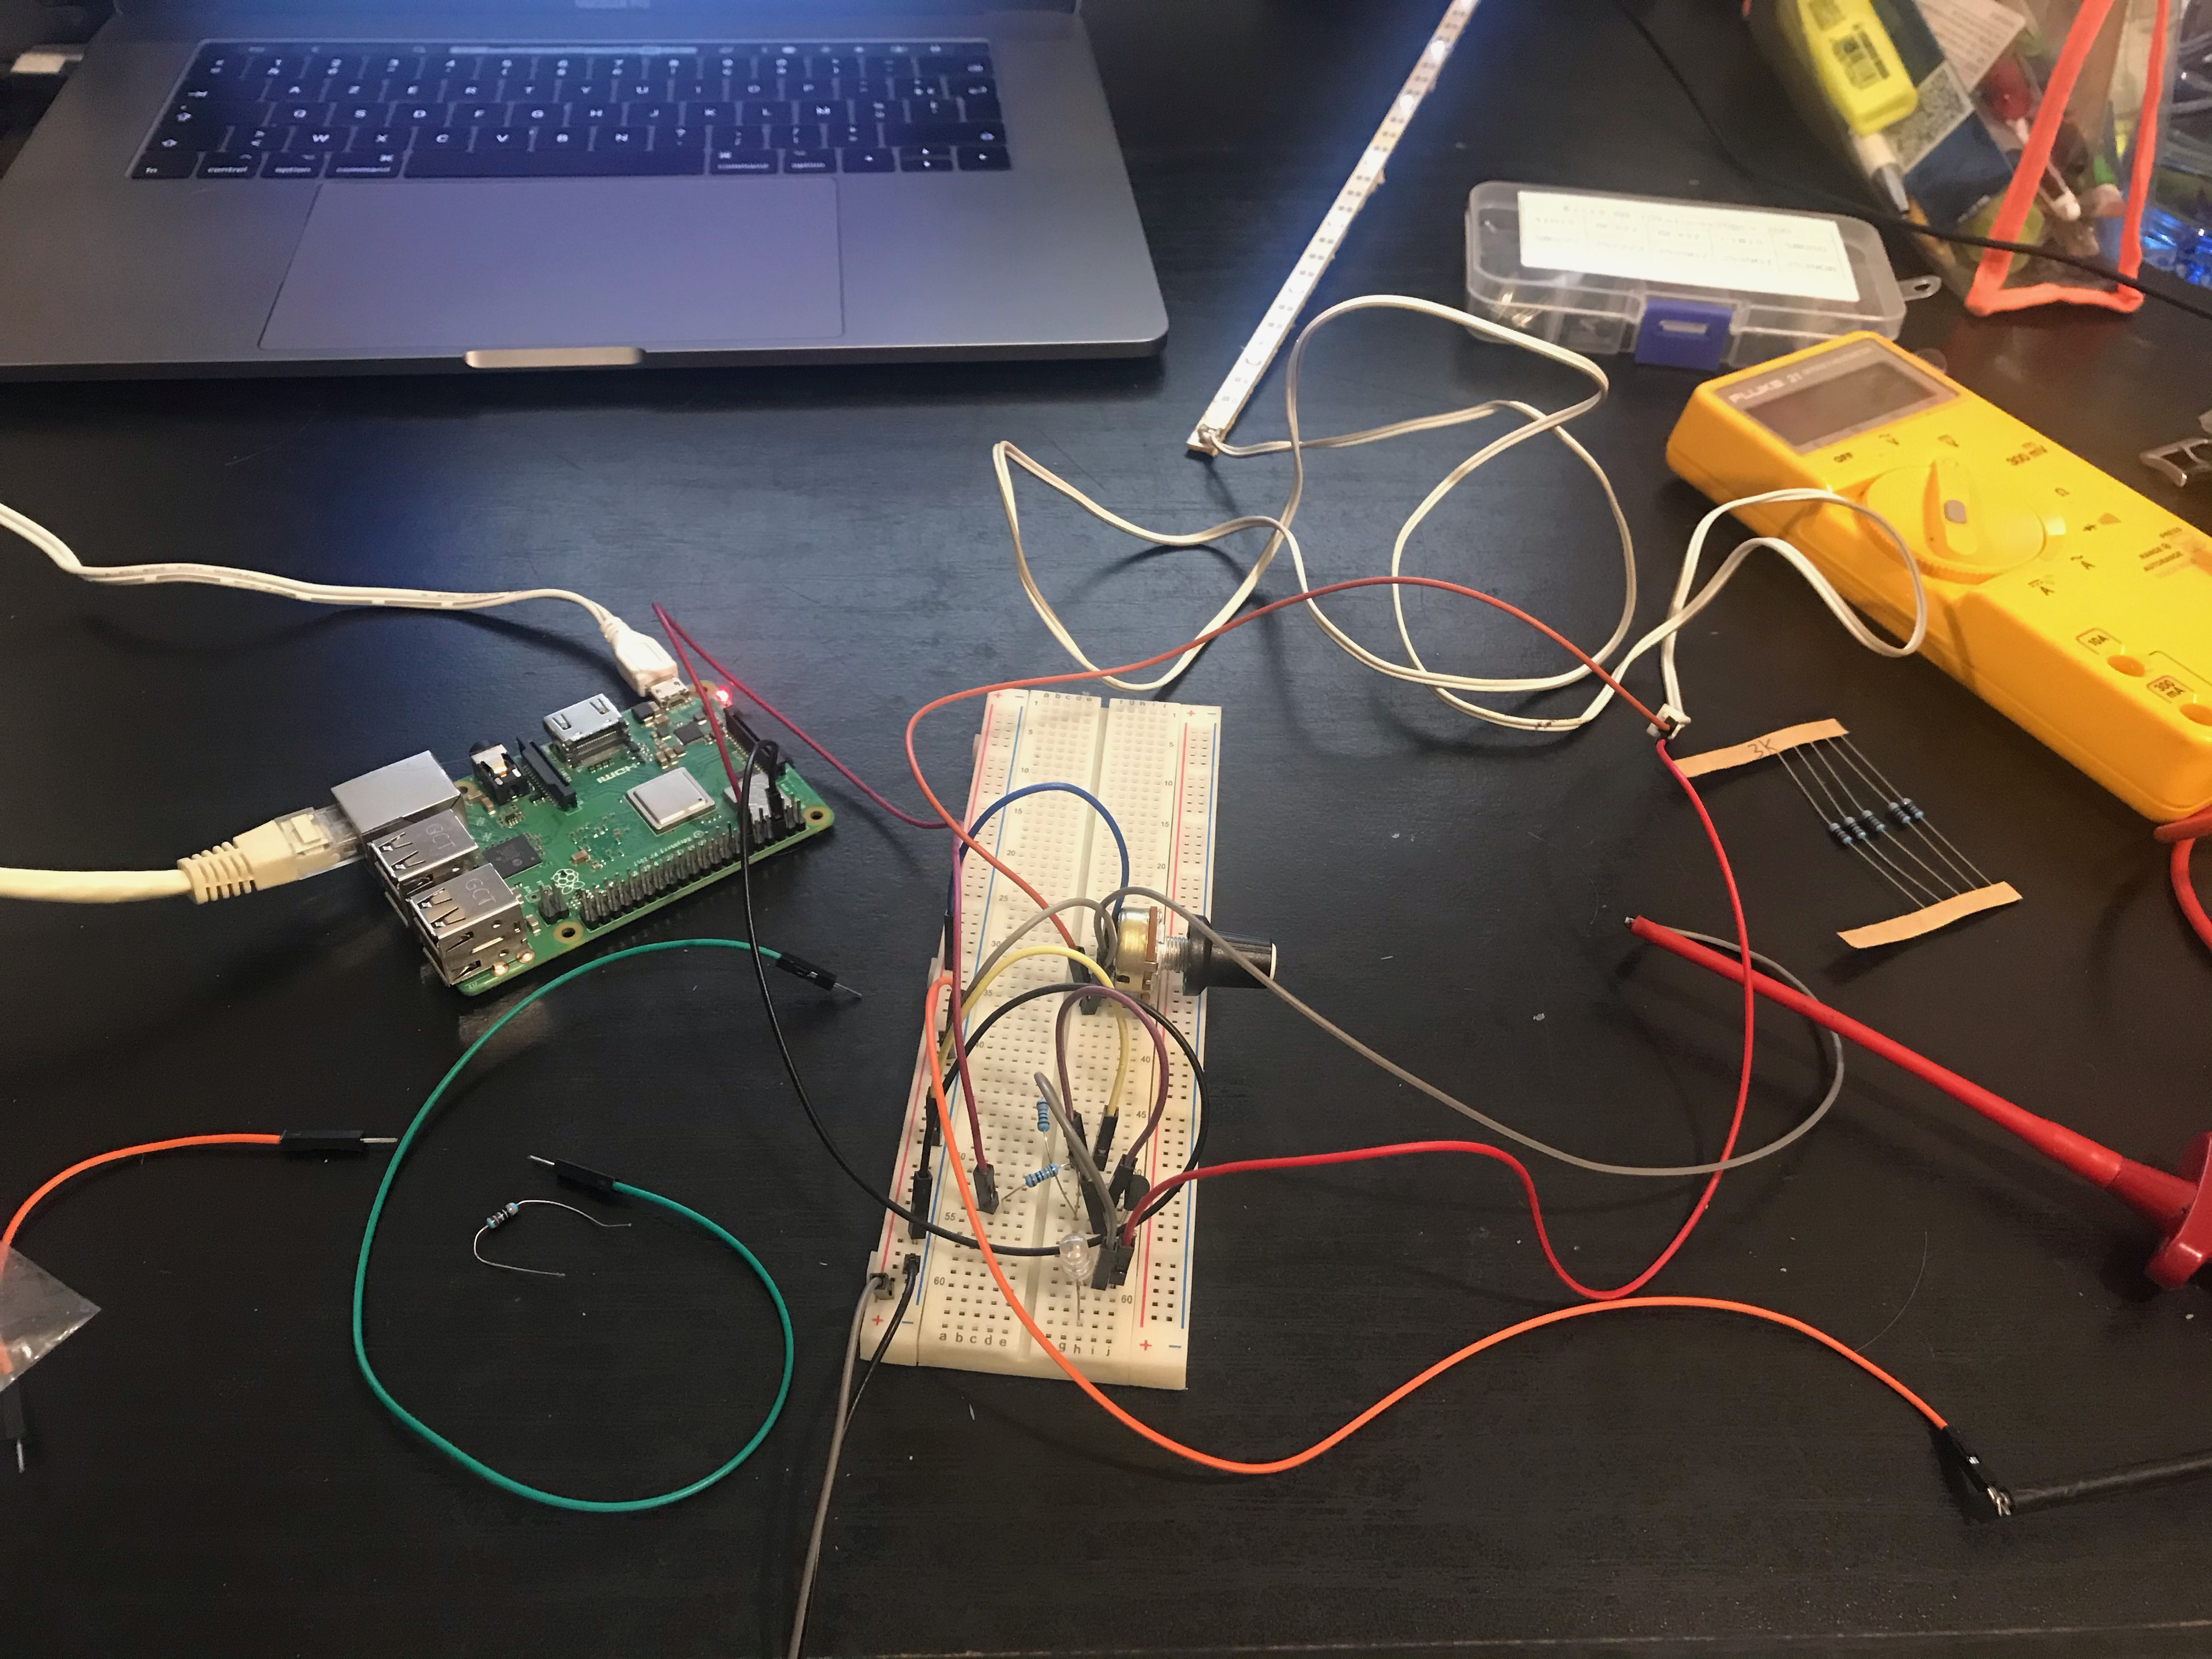
\includegraphics[height=3.125000in, keepaspectratio=true]{./fig/Camera_setup/Light/White_Led_Strips/Test_setup_ledstrip.jpeg}
\caption{White led strips test circuit.}
\label{fig:setup:whiteled:circuit}
\end{figure}

	\subsubsection{Adressable Color Changeable Led Strip}

		A third option of lighting is playing with the colors of the light. to archieve this a setup will be created with a single adressable light strip where the color and led can be freely chosen. 
		To assign a color which works best; a study is made to find the wavelengths where the light reflects most on the used materials of the tool. This can be found in  Light Reflection

From all these settings the single adressable led strip was chosen due to the amount of options this creates. This choice is documented in future tests which will be discussed in section ........... . The led strip were mounted on metal strips which provided high adjustability. This made it possible to get lighting on different parts of the tool insert what makes later research easier. In Figure ..... the light configuration is displayed for a partly worn tool.
	
	insert tool with reflection
	
	As seen on this render there are a lot of options with this setup. Each led strip can rotate and fifteen leds can be individually set to a color. The arc keeps a consistent distance between the led and the insert. 

\section{Datasets}
A separation is made between hand made datasets and automated datasets because they take a very different approach and produce very differing results.

	\subsection{Handmade datasets}

The following datasets where produced using a microscopic camera to take pictures of single inserts all placed under the camera by hand. The initial dataset is produced by Sirris 

		\subsubsection{initial dataset}

			The initial dataset where the images made by a microscopic camera at Sirris. These pictures were taken for the measurement of the tool wear. This dataset provided the labels for the first 5 batches labeled with 00x as batch number. This data was directly saved from the output of the microscopic camera. For this reason there is a lot of extra information on the picture as seen in Figure \ref{fig:dataset:initial}. The labels for this dataset where sorted with or without tag on the insert but the transcription code was lost. For example the insert had a mark on one side and no mark on the other side and the labels had a value for some insert a and some insert b. For this combination it wasn't known whether label a was the side with the mark or the other way round.
			
			Since the labels weren't clear and the images where not optimal these inserts where all done again in a new hand made dataset called the second handmade dataset.
			
			\begin{figure}[hbtp]
			\centering
			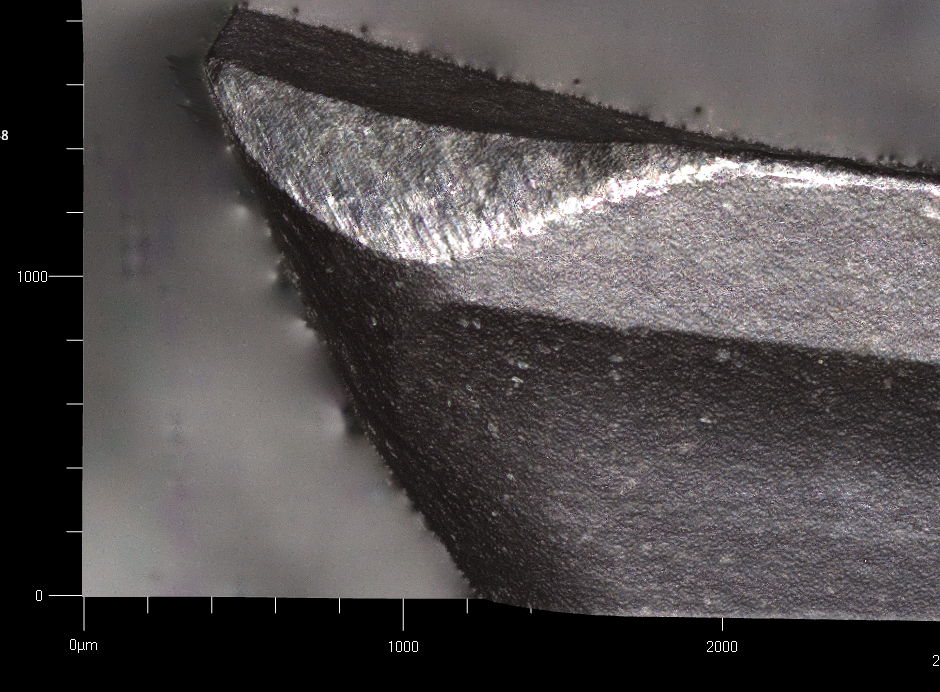
\includegraphics[scale=0.2]{fig/Vision/Dataset/handmade_datasets/initial_dataset/initial dataset pictuer.PNG}
			\caption{Example of initial dataset}
			\label{fig:dataset:initial}
			\end{figure}

\paragraph{Form}

The dataset given where taken with a microscopic camera at Sirris. These images were in good lighting conditions for the measurement, but had a lot of extra "unwanted" features on it. The background was very like the wear and the rest of the tool insert. 

Every insert that was measured had a little mark on one side to mark the a and b. Sadly the information about what the marker meant is lost. To find the corresponding values, the inserts where once again put through a microscopic camera and the new pictures where compared against the old ones. 

While again checking the inserts out, a new dataset is created since this didn't ask much more time. During this proces there is also a new way of separating the sides of the inserts. There is a bullet at one side on every insert. This is an easy way to recognise a side and wont dissapear like the marker line. 
			
		\subsubsection{Second handmade dataset}
		\label{sec:impl:ds:shm}

			A second dataset was made to compare the pictures with the previous dataset. This is done to verify the images and the results and to determine what the marker meant. This dataset also handles the first 5 batches labeled with 00x. For this dataset a setup much like the setup with the desk light was used but instead of lighting with the desk light only the light from the camera was used.
			
			A second handmade dataset is made to compare with the first dataset and get to know what the stripes mean on the first dataset which was used to measure the wear.

		The next setup is used:

		The light came primarely from the camera itself which was set in the first brightness setting. 

		The camera was located at a distance of 2cm between the housing and the measured point on the insert. The housing starts at the black part; not the plexi glass protector. 

		During the making of this dataset the inserts where labeled with bullet or no bullet. This was not setup this way in the first place; instead there was a marker line on the insert. This marker line is also noted in the labels of the dataset.

		An "s" means it is with a marker line. A

		\begin{tabular}{ |l|l| }
			\hline
 				symbol & explanation \tabularnewline
			\hline
			\hline
				 s & side with marker line \tabularnewline
			\hline
				 n & side without marker line \tabularnewline
			\hline
				 batch number & number specified on the box in which the inserts are kept \tabularnewline
			\hline
				 plate number & number specified inside the box; this goes from 1 to 10 per batch \tabularnewline
			\hline
		\end{tabular}


		The naming of the dataset is the following

		b\_\textless{}batch number\textgreater{}\_p\_\textless{}plate number\textgreater{}\_\textless{}identifier of side\textgreater{}

		After looking at the pictures of the datasets it can be confirmed that the 'b' side of the inserts is the side with the mark on. 

		This can be seen on the folowing two pictures whis correspond. The first one is from the first dataset, the second from the second dataset.

			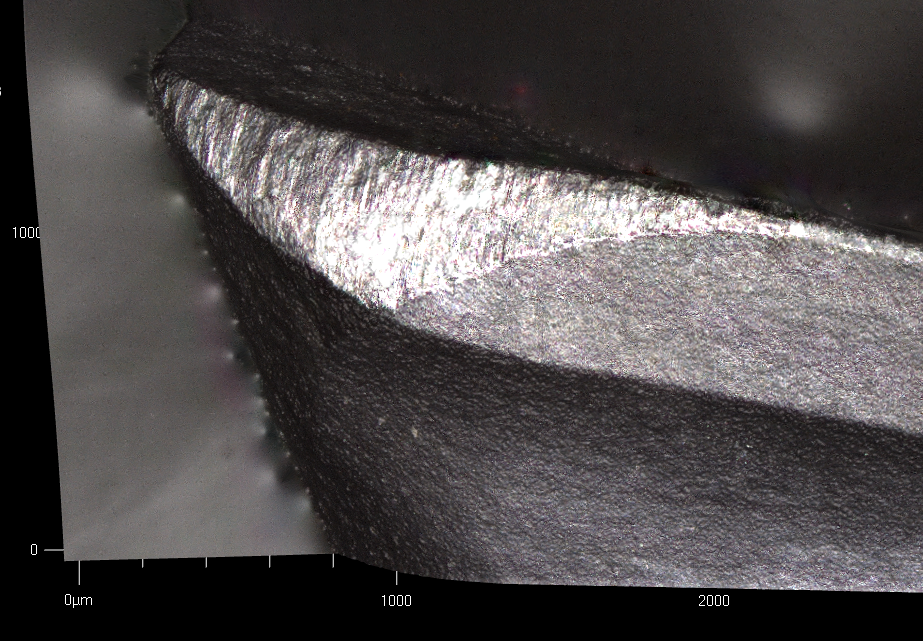
\includegraphics[height=2.083333in, keepaspectratio=true]{./fig/Vision/Dataset/handmade_datasets/Second_handmade_dataset/t50b-img.PNG}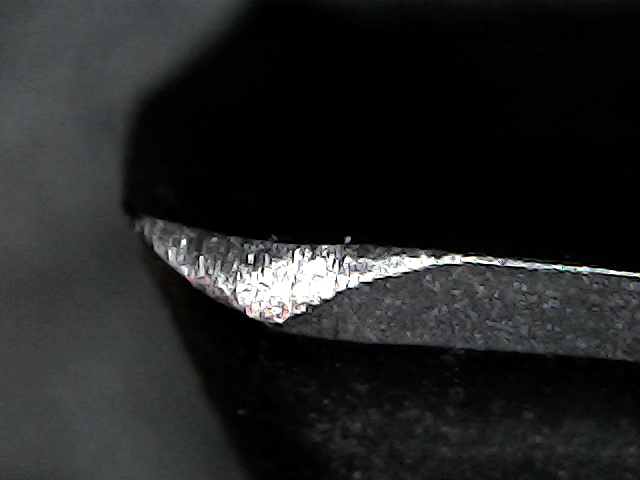
\includegraphics[height=2.083333in, keepaspectratio=true]{./fig/Vision/Dataset/handmade_datasets/Second_handmade_dataset/b_005_p_010_s.jpg}
	
		\subsubsection{second initial dataset}

			The second initial dataset was made with the inserts from batches 11 to 19 labeled with 01x. Here the images where taken with the same microscope as the first initial dataset but instead of phtotographing only the one insert at a time; two inserts are photographed per shot.
			
With the second number of inserts (batch 11 to 19) another dataset was created for measurement.

Since the photo's where labeled with two inserts at a time; the images taken where not relevant for the data processing and were not saved

The distance for these inserts is measured between the line connecting the two highest points visible on the insert and the outer most point of the wear area.

	\subsection{Automated datasets}

	The hand made datasets are not scalable for a hundred or even a thousand inserts so a way of automatically creating datasets was researched. For this creation the past sections were used to create a setup and lighting conditions. With those things figured out a program was written to control the setup and save the taken images in a logical order. This process took a lot of test tries to find out a good camera position which will be handled first. After that the two main created datasets will be discussed.
	
	
	\begin{enumerate}[1]
	\item birthday dataset
		\begin{enumerate}[a]
		\item conducted tests
		\end{enumerate}
	\item Spaghetti dataset
		\begin{enumerate}[a]
		\item conducted tests
		\end{enumerate}
	\end{enumerate}


		\subsubsection{Camera position}
		
		With the help of 
		In this section the best camera position will be defined  for the creation of the dataset. Top view as well as side view will be tested.

		\paragraph{Side camera position}

For these tests the first four plates of batch 004 are used. The lighting is red light coming from the addressable led strips that shine from different directions. This setup can be seen on Figure \ref{fig:dataset:cameraposition:side}.

\begin{figure}[hbtp]
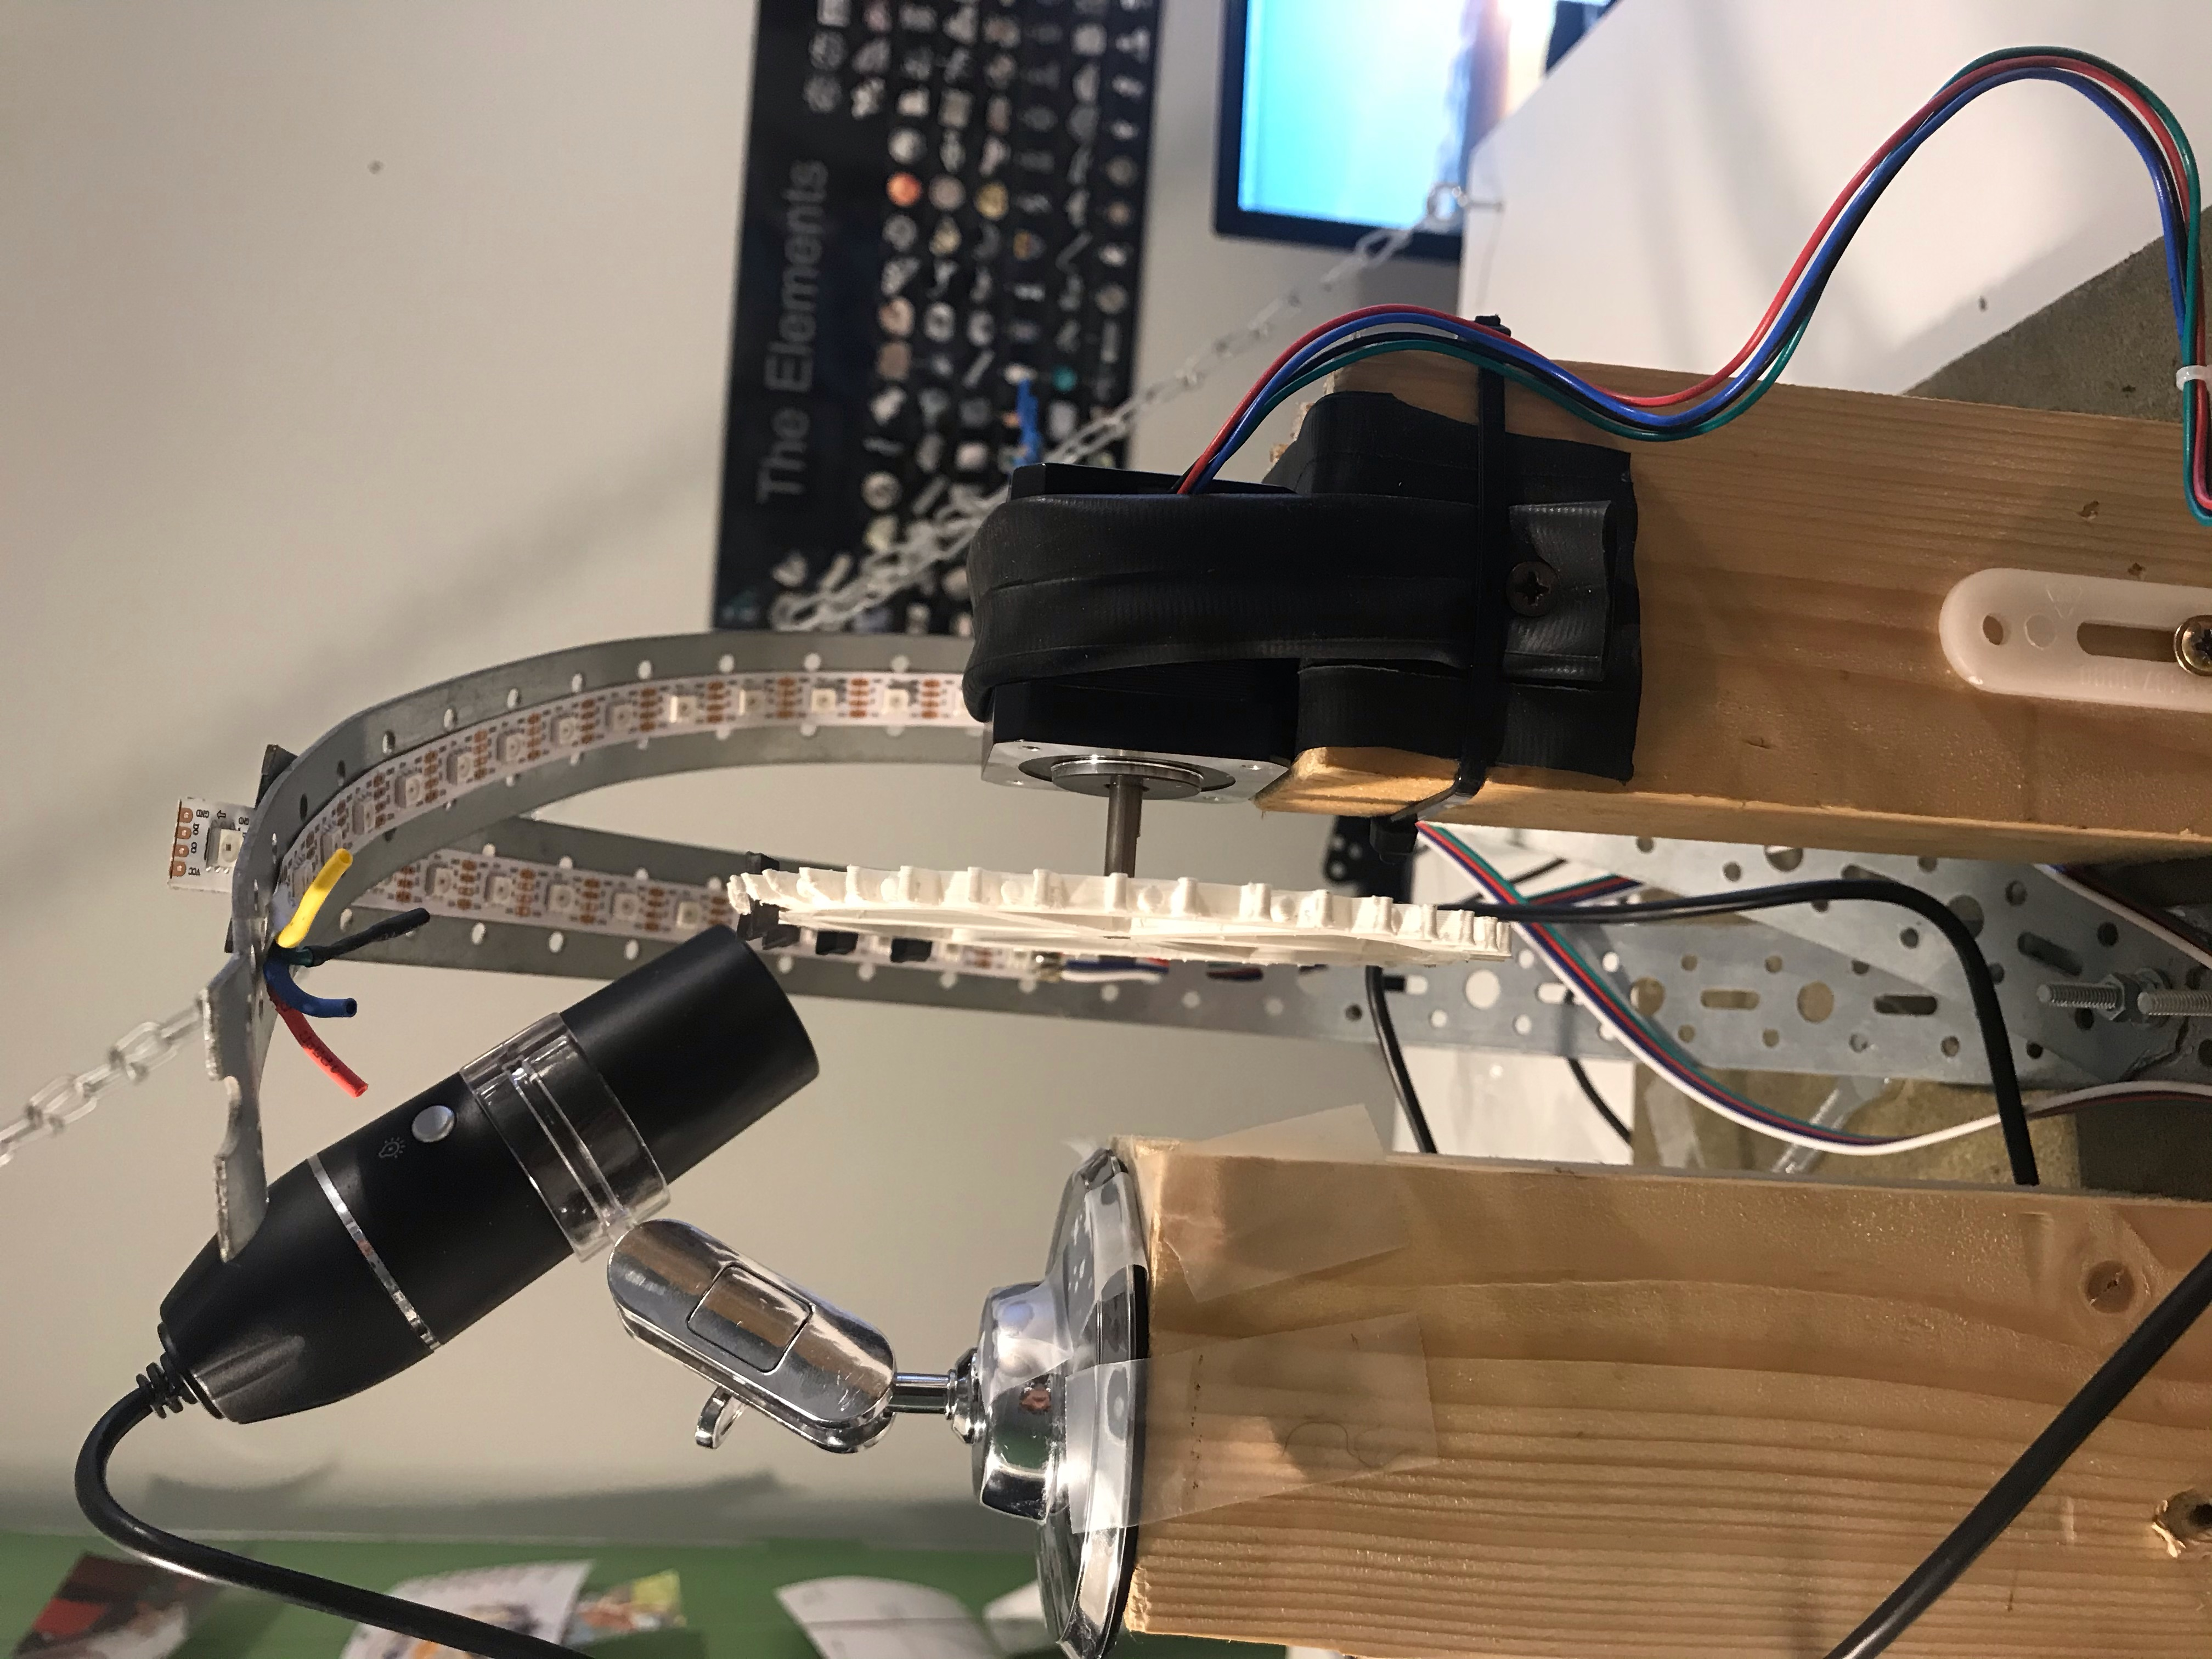
\includegraphics[width=4.166667in, keepaspectratio=true,angle=270]{./fig/Vision/Dataset/automated_datasets/1_check_camera_position/1_camera_position_side/achter2.jpeg}
\caption{Camera setup for testing the camera angle.}
\label{fig:dataset:cameraposition:side}
\end{figure}

Due to the problems with the arduino communications described here the first dataset wasn't successfull because the leds didn't turn on when the photo's where taken. So the results are all black pictures with al little shadow of the insert caused by the polluting light. 

By putting a delay before sending a command to the Arduino to provide the wanted lighting conditions. Although this was a very long process the results are way better than the ones from the first take on this camera setup. 

The results of this test setup can be found in Figure \ref{fig:dataset:cameraposition:side:results}. The insert is lighted with two corresponding leds coming from the two led strips. On the left is the result for led number 8; in the middle led number 9 and on the right led number 10. This lightens the worn area very good. Although the background is lighted as well and makes it harder to only see the worn area. On this we can build the first dataset but first some other camera positions are tested.

\begin{figure}
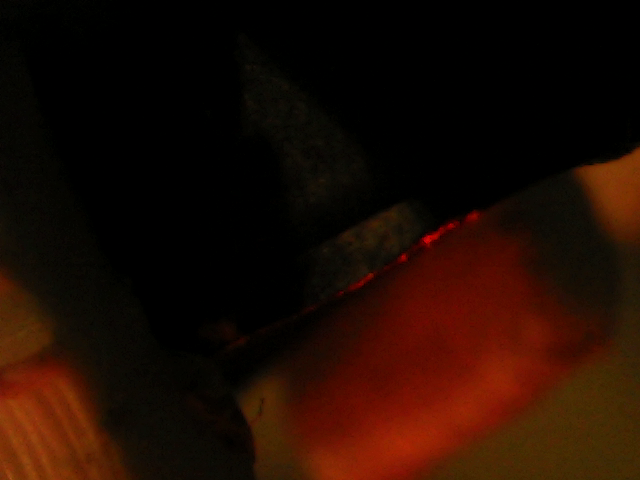
\includegraphics[width=.3\textwidth, keepaspectratio=true]{./fig/Vision/Dataset/automated_datasets/1_check_camera_position/1_camera_position_side/p3_l8.png}\hfill
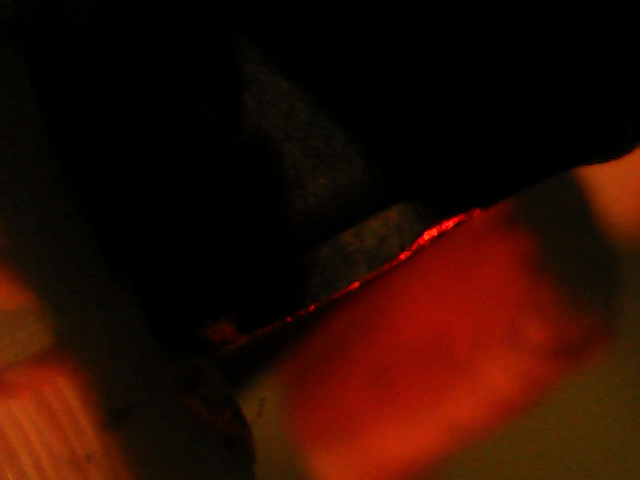
\includegraphics[width=.3\textwidth, keepaspectratio=true]{./fig/Vision/Dataset/automated_datasets/1_check_camera_position/1_camera_position_side/p3_l9.png}\hfill
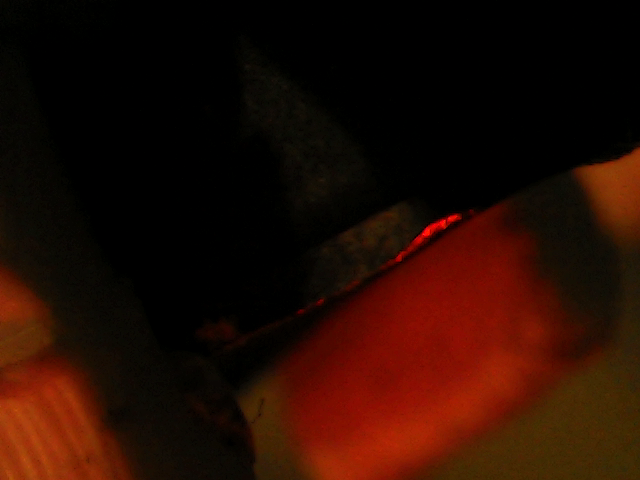
\includegraphics[width=.3\textwidth, keepaspectratio=true]{./fig/Vision/Dataset/automated_datasets/1_check_camera_position/1_camera_position_side/p3_l10.png}
\caption{Side camera view for led 8 through 10 listed from left to right.}
\label{fig:dataset:cameraposition:side:results}
\end{figure}

		\paragraph{Top camera position}

The same inserts where used 04 -\textgreater{} 1until 5. 

Every pair of led is lighted separately to generate the photo's 
extra documents of the results in the folders images/dataset/.....

The second test was conducted with the camera mounted a little more to the top of the inserts. This made the reflection from the worn area to the camera better. 

For this test the issue with the arduino communication was resolved by changing the input delay from the serial input reader.The following pictures where the result. 
Like on the previous test one picture was taken for every two leds of the strip with red light. for batch number 4 insert 3 this time with leds 5,6 and 7 turned on since the position of the camera relative to the leds is changed.

\begin{figure}
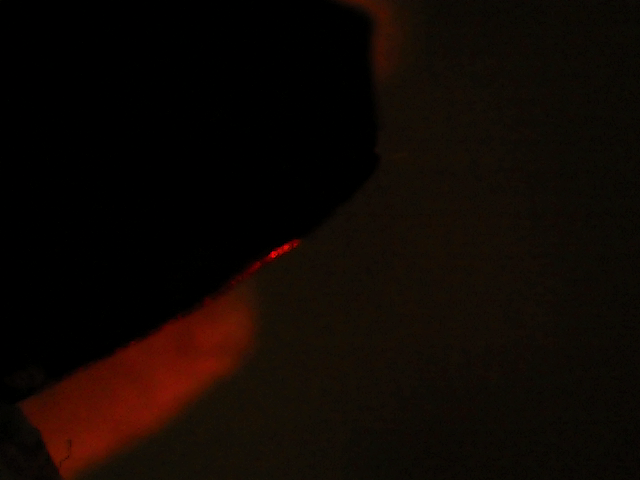
\includegraphics[width=0.32\textwidth, keepaspectratio=true]{./fig/Vision/Dataset/automated_datasets/1_check_camera_position/2_camera_position_top/p3_l5.png}\hfill
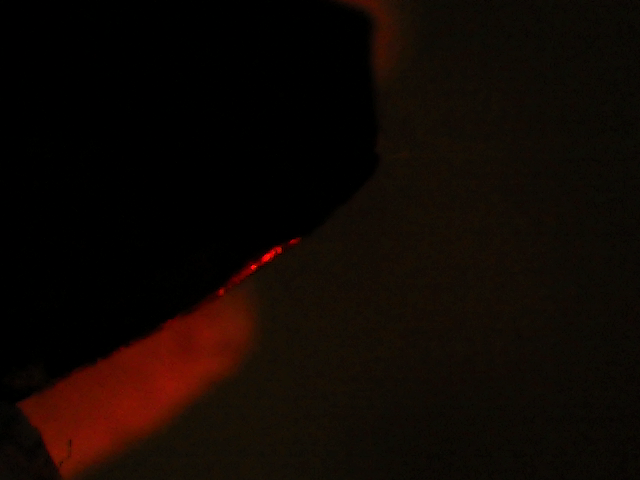
\includegraphics[width=.32\textwidth, keepaspectratio=true]{./fig/Vision/Dataset/automated_datasets/1_check_camera_position/2_camera_position_top/p3_l6.png}\hfill
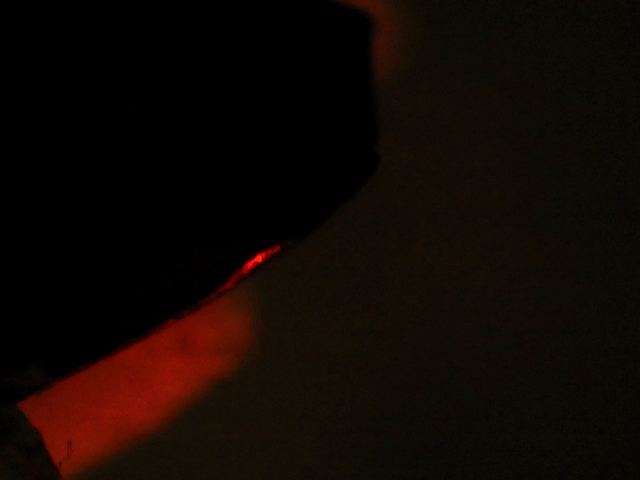
\includegraphics[width=.32\textwidth, keepaspectratio=true]{./fig/Vision/Dataset/automated_datasets/1_check_camera_position/2_camera_position_top/p3_l7.png}
\caption{Top camera view for leds 5 through 7 listed from left to right.}
\label{fig:dataset:cameraposition:top:results}
\end{figure}

On this data we can see the leds going up on the insert wear area. Which is what we tried to obtain. Now the leds are mapped to specific positions on the inserts and the amount of leds that need to be turned on for taking pictures can be reduced so no extra time is wasted. 

		\subsection{Created datasets}

The full datasets will be discussed in this page where firstly the dataset is documented and after that the tests that lead to this dataset are discussed.

\subsubsection{Birthday dataset}

Created a dataset on 27/11/2020 with a part of the given inserts for every possible color and led setting where pictures are taken from two separate led strips and every led one after another. This is done for white, red, green and blue colors. 

Done for batch 1 to 11

On November 27th a new dataset is created where for every plate 91 pictures are taken. 

The following pictures are available for the dataset:

\begin{itemize}
\item 1 picture with all leds on white
\item 30 pictures with red lighting; 15 of led strip A and 15 of led strip B
\item 30 pictures with blue lighting; 15 of led strip A and 15 of led strip B
\item 30 pictures with green lighting; 15 of led strip A and 15 of led strip B
\end{itemize}


The brightness is set to 80\% for all lights to make sure to not clip against the top values.

The dataset consists of 120*91 photos of 60 inserts with 120 worn sides. After 120 the quality was evaluated and the red, green and blue colors didn't seem to add more information to the pictures. 

In this dataset, there are some pictures unusable. As some worn areas are not even in the frame. Some to the left side and some to the right side. The placement of the wheel which holds the plates wasn't checkt thoroughly.

The setup for creating this dataset was as follows:
\begin{figure}[hbtp]
\centering
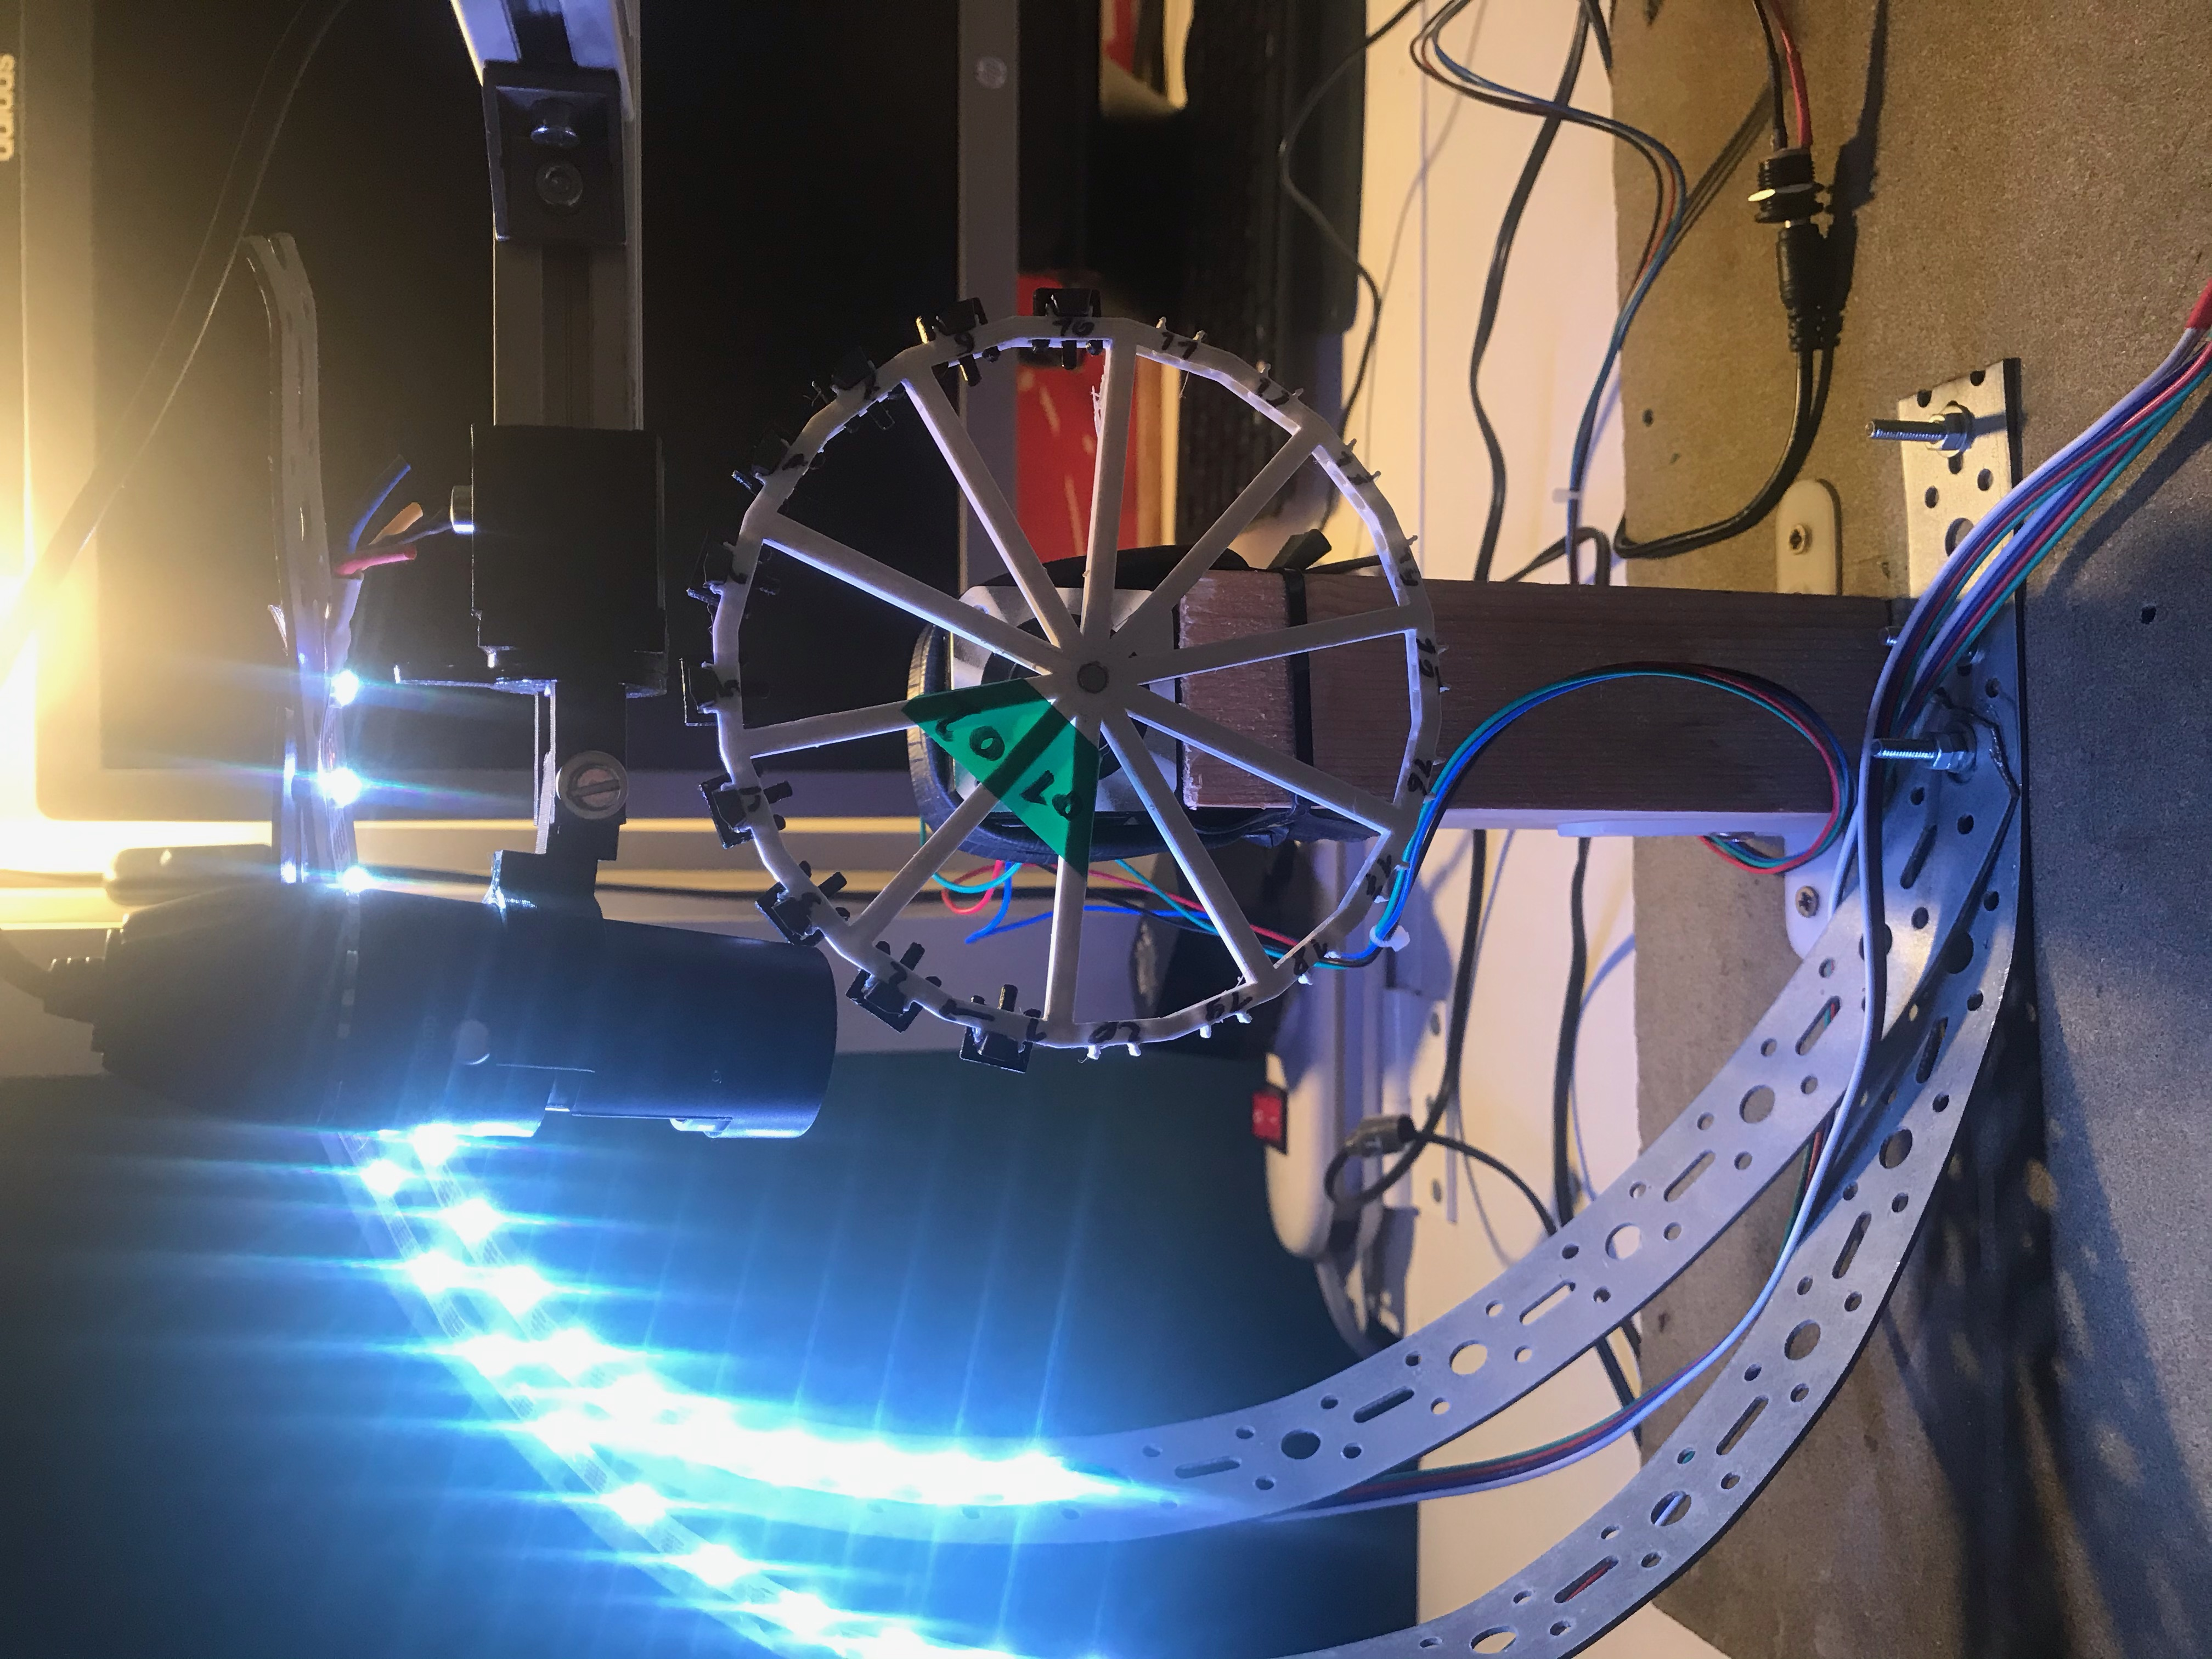
\includegraphics[width=4.166667in, keepaspectratio=true, angle=270]{./fig/Vision/Dataset/automated_datasets/2_created_datasets/1_Birthday_dataset/IMG_9282.jpeg}
\caption{some caption}
\end{figure}

Here two ledstrips where mounted and pointed at the photographed insert. The inserts where attached to the wheel with black clips 3D printed with PETG. This was shosen above white clips to lower the light reflections into the camera lens. This was a problem in previous setups. 

Also a sturdy camera mount was fabricated out off metal profiles and 3D printed parts to get better notice of the placement of the camera opposed to the insert. 

The image taking process took about 1 minute per batch because of the amount of pictures taken. Since time was limited and the setup wasn't yet perfect we decided to only run 60 inserts through it. These where from batches 1 to 11. 

Sample pictures of this dataset can be found underneath. 

For every led one picture is taken. These images can be put together to create images on a full spectrum of leds and take out the best conditions. 

This can be done by inserting the images as different channels in the model.



The next pictures are from batch 3 insert 5 with led 6 turned on for both led strips and four colors.

\begin{figure}[hbtp]
\centering
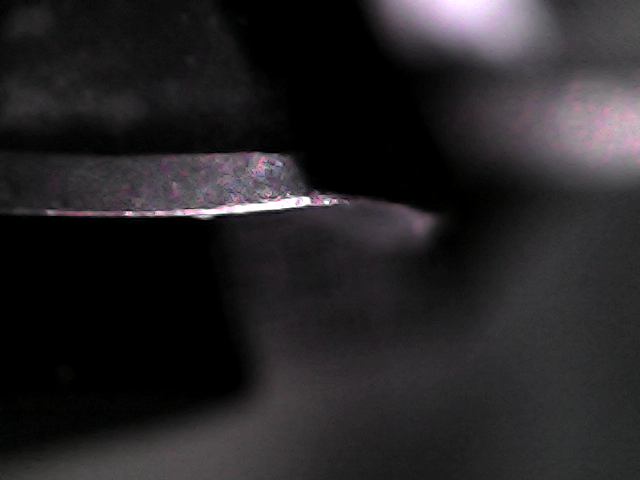
\includegraphics[width=.3\textwidth, keepaspectratio=true]{./fig/Vision/Dataset/automated_datasets/2_created_datasets/1_Birthday_dataset/b_003_p_005_l_000_b.png}
\caption{Fully lit example for insert 5 from batch 3.}
\end{figure}

\begin{figure}
	\begin{subfigure}{0.24\textwidth}
		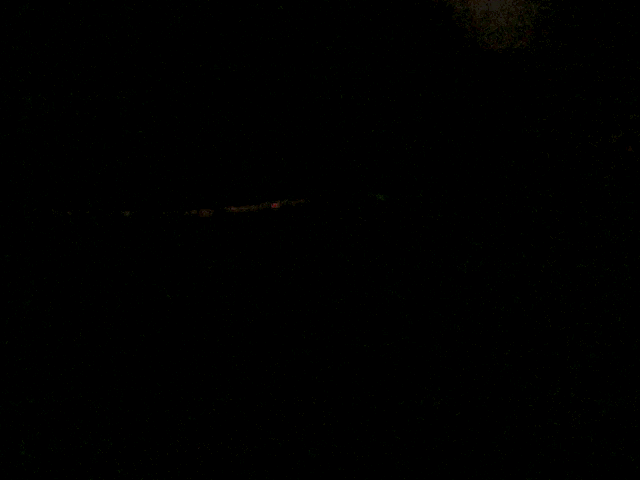
\includegraphics[width=\linewidth, keepaspectratio=true]{./fig/Vision/Dataset/automated_datasets/2_created_datasets/1_Birthday_dataset/b_003_p_005_b_l_006_red_A.png}
		\caption{Red}
	\end{subfigure}
	\hspace*{\fill}
	\begin{subfigure}{0.24\textwidth}
		
\includegraphics[width=\linewidth, keepaspectratio=true]{./fig/Vision/Dataset/automated_datasets/2_created_datasets/1_Birthday_dataset/b_003_p_005_b_l_006_green_A.png}
		\caption{Green}
	\end{subfigure}
	\hspace*{\fill}
	\begin{subfigure}{0.24\textwidth}
		
\includegraphics[width=\linewidth, keepaspectratio=true]{./fig/Vision/Dataset/automated_datasets/2_created_datasets/1_Birthday_dataset/b_003_p_005_b_l_006_blue_A.png}
		\caption{Blue}
	\end{subfigure}
	\hspace*{\fill}
	\begin{subfigure}{0.24\textwidth}
		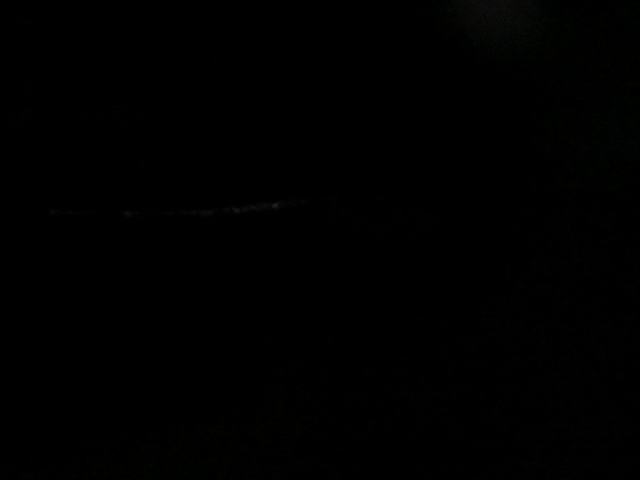
\includegraphics[width=\linewidth, keepaspectratio=true]{./fig/Vision/Dataset/automated_datasets/2_created_datasets/1_Birthday_dataset/b_003_p_005_b_l_006_white_A.png}
		\caption{White}
	\end{subfigure}
\caption{Red, green, blue and white lighting on insert 5 from batch 3 led strip one. Left to right respectively}
\end{figure}

\begin{figure}
	\begin{subfigure}{0.24\textwidth}
		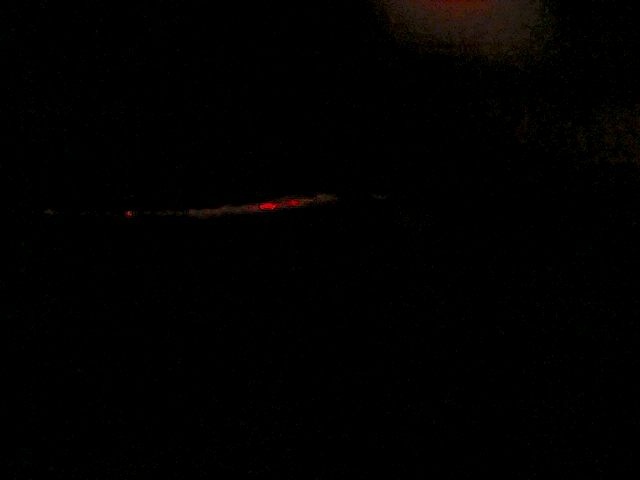
\includegraphics[width=\linewidth, keepaspectratio=true]{./fig/Vision/Dataset/automated_datasets/2_created_datasets/1_Birthday_dataset/b_003_p_005_b_l_006_red_B.png}
		\caption{Red}
	\end{subfigure}
	\hspace*{\fill}
	\begin{subfigure}{0.24\textwidth}
		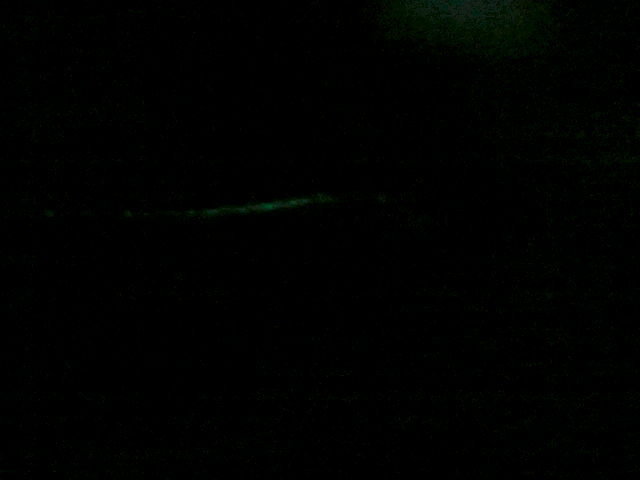
\includegraphics[width=\linewidth, keepaspectratio=true]{./fig/Vision/Dataset/automated_datasets/2_created_datasets/1_Birthday_dataset/b_003_p_005_b_l_006_green_B.png}
		\caption{Green}
	\end{subfigure}
	\hspace*{\fill}
	\begin{subfigure}{0.24\textwidth}
		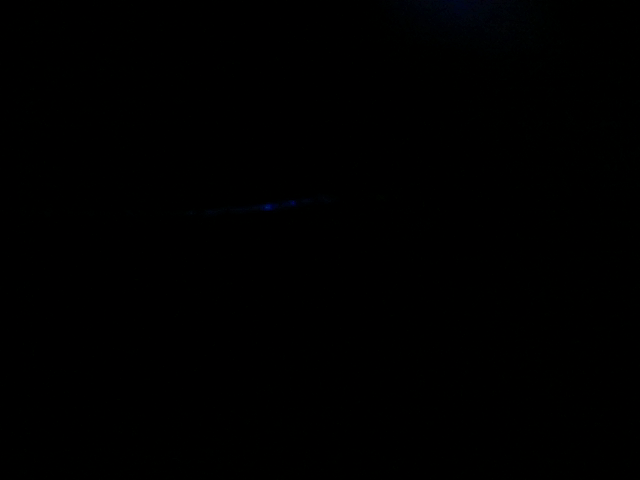
\includegraphics[width=\linewidth, keepaspectratio=true]{./fig/Vision/Dataset/automated_datasets/2_created_datasets/1_Birthday_dataset/b_003_p_005_b_l_006_blue_B.png}
		\caption{Blue}
	\end{subfigure}
	\hspace*{\fill}
	\begin{subfigure}{0.24\textwidth}
		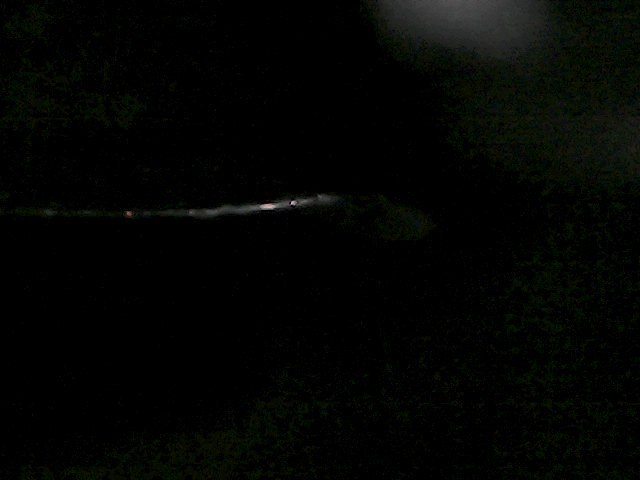
\includegraphics[width=\linewidth, keepaspectratio=true]{./fig/Vision/Dataset/automated_datasets/2_created_datasets/1_Birthday_dataset/b_003_p_005_b_l_006_white_B.png}
		\caption{White}
	\end{subfigure}
\caption{Red, green, blue and white lighting on insert 5 from batch 3 led strip two. Left to right respectively.}


\end{figure}

On these pictures we can see only red and white are visible and the B led strip wasn't visible. For this purpose the color of the wheel is changed to Black for less reflections. In the next dataset only white and red will be used for lighting. 

\subparagraph{Errors}

\begin{figure}[hbtp]
	\begin{subfigure}{0.49\textwidth}
		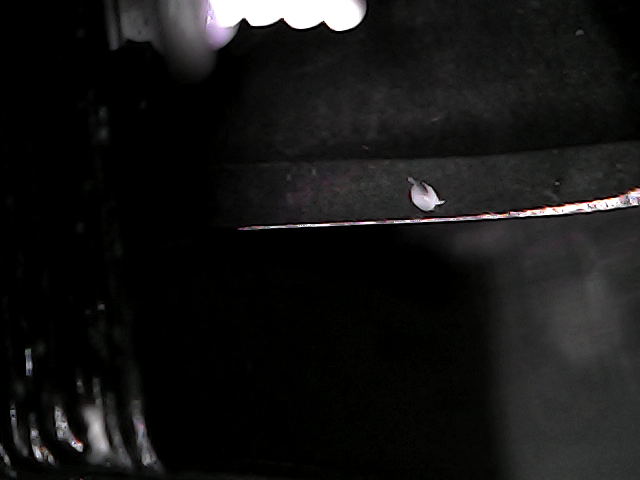
\includegraphics[width=\linewidth, keepaspectratio=true]{./fig/Vision/Dataset/automated_datasets/2_created_datasets/1_Birthday_dataset/b_003_p_010_l_000_nb.png}
		\caption{Insert out of frame left.}
	\end{subfigure}
	\hspace*{\fill}
	\begin{subfigure}{0.49\textwidth}
		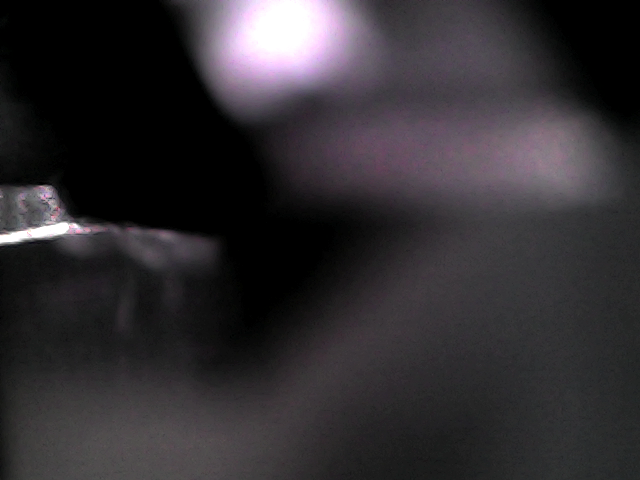
\includegraphics[width=\linewidth, keepaspectratio=true]{./fig/Vision/Dataset/automated_datasets/2_created_datasets/1_Birthday_dataset/b_003_p_010_l_000_b.png}
		\caption{Insert out of frame right.}
	\end{subfigure}
	\hspace*{\fill}
	\begin{subfigure}{0.49\textwidth}
		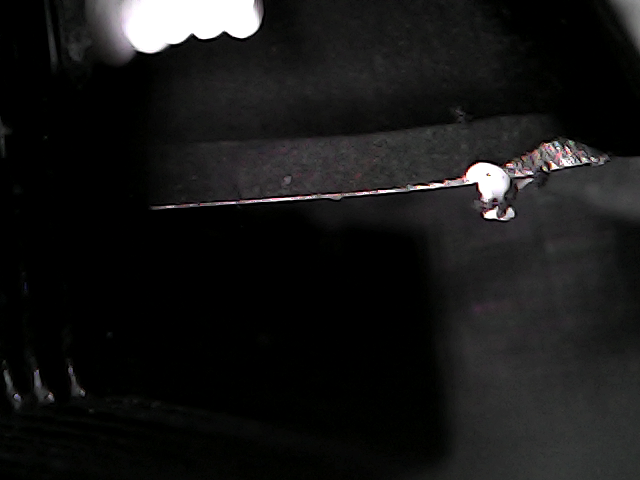
\includegraphics[width=\linewidth, keepaspectratio=true]{fig/Vision/Dataset/automated_datasets/2_created_datasets/1_Birthday_dataset/error/b_003_p_007_l_000_nb.png}
		\caption{Plastic on insert.}
	\end{subfigure}
	\hspace*{\fill}
	\begin{subfigure}{0.49\textwidth}
		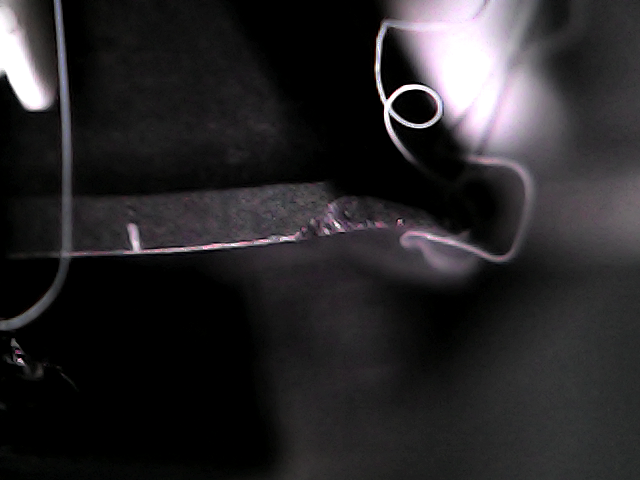
\includegraphics[width=\linewidth, keepaspectratio=true]{fig/Vision/Dataset/automated_datasets/2_created_datasets/1_Birthday_dataset/error/b_005_p_006_l_000_b.png} 
		\caption{Bad lighting angle and plastic.}
	\end{subfigure}
	\caption{left: batch 3 insert 10 the side without bullet is off to the right side. right: batch 3 insert 10 The side with bullet. Is far off to the left side.}
\caption{a. Plastic occludes the worn area. batch 3 plate 7 no bullet:  had restants of 3D print plastic on worn area}
\label{fig:dataset:birthday:error}
\end{figure}

batch 5 plate 6 no bullet lighting not good

batch 5 plate 6 bullet has string from 3D printing on wear area
batch 11 plate 5 bullet had hair on wear area

\subsubsection{spaghetti dataset}

After the Birthday dataset a new dataset was created using the things learned from that. Now the amount of leds driven is reduced to 5 leds. Where led 6 to 11 is used to lighten the inserts. 

only the colors white and red are used for this dataset. Previously was discussed that the red color could have an influence on the reflection of the carbide of which the inserts are made see light reflection.

\subsection{Dataset explanation}

For every insert, two pictures are taken. One with leds 6 to 11 on red and one with these leds white. This was experimentally found to be the best setting for reflecting the light off the worn area and into the camera. 

Turning on a led to much on the upper bounary will lighten the side of the insert which isn't of much use in this paper. Turining on a led to much on the bottom boundary makes the background very bright which supports unnessesary information.



The images are separated in a folder for every insert named with batch number and insert number:

batch\_aaa\_plate\_bbb where aaa is the batch number and bbb is the insert number.

Images are named with their settings, batch number and insert number:

b\_aaa\_p\_bbb\_l\_006-011\_color\_bullet.png 

where 

\begin{itemize}
\item aaa is the batch number; 
\item bbb is the plate number, 
\item 006-011 are the leds that turned on at the same time; 
\item color is the color: red or white
\item bullet is the appearance of a bullet on the side of the inset and has values of b for bullet or nb for no bullet.
\end{itemize}


The dataset inserts consisted of a few different types and coatings. 



\subsection{Setup}

The setup used is exactly the same as on the Birthday dataset where the camera is positioned as much to the top as possible. This can be seen on the picture:

Here we can see the led strips are a little bit twisted and are positioned very close to each other. This made the reflection better and should result in beter outcome of the algorithm.



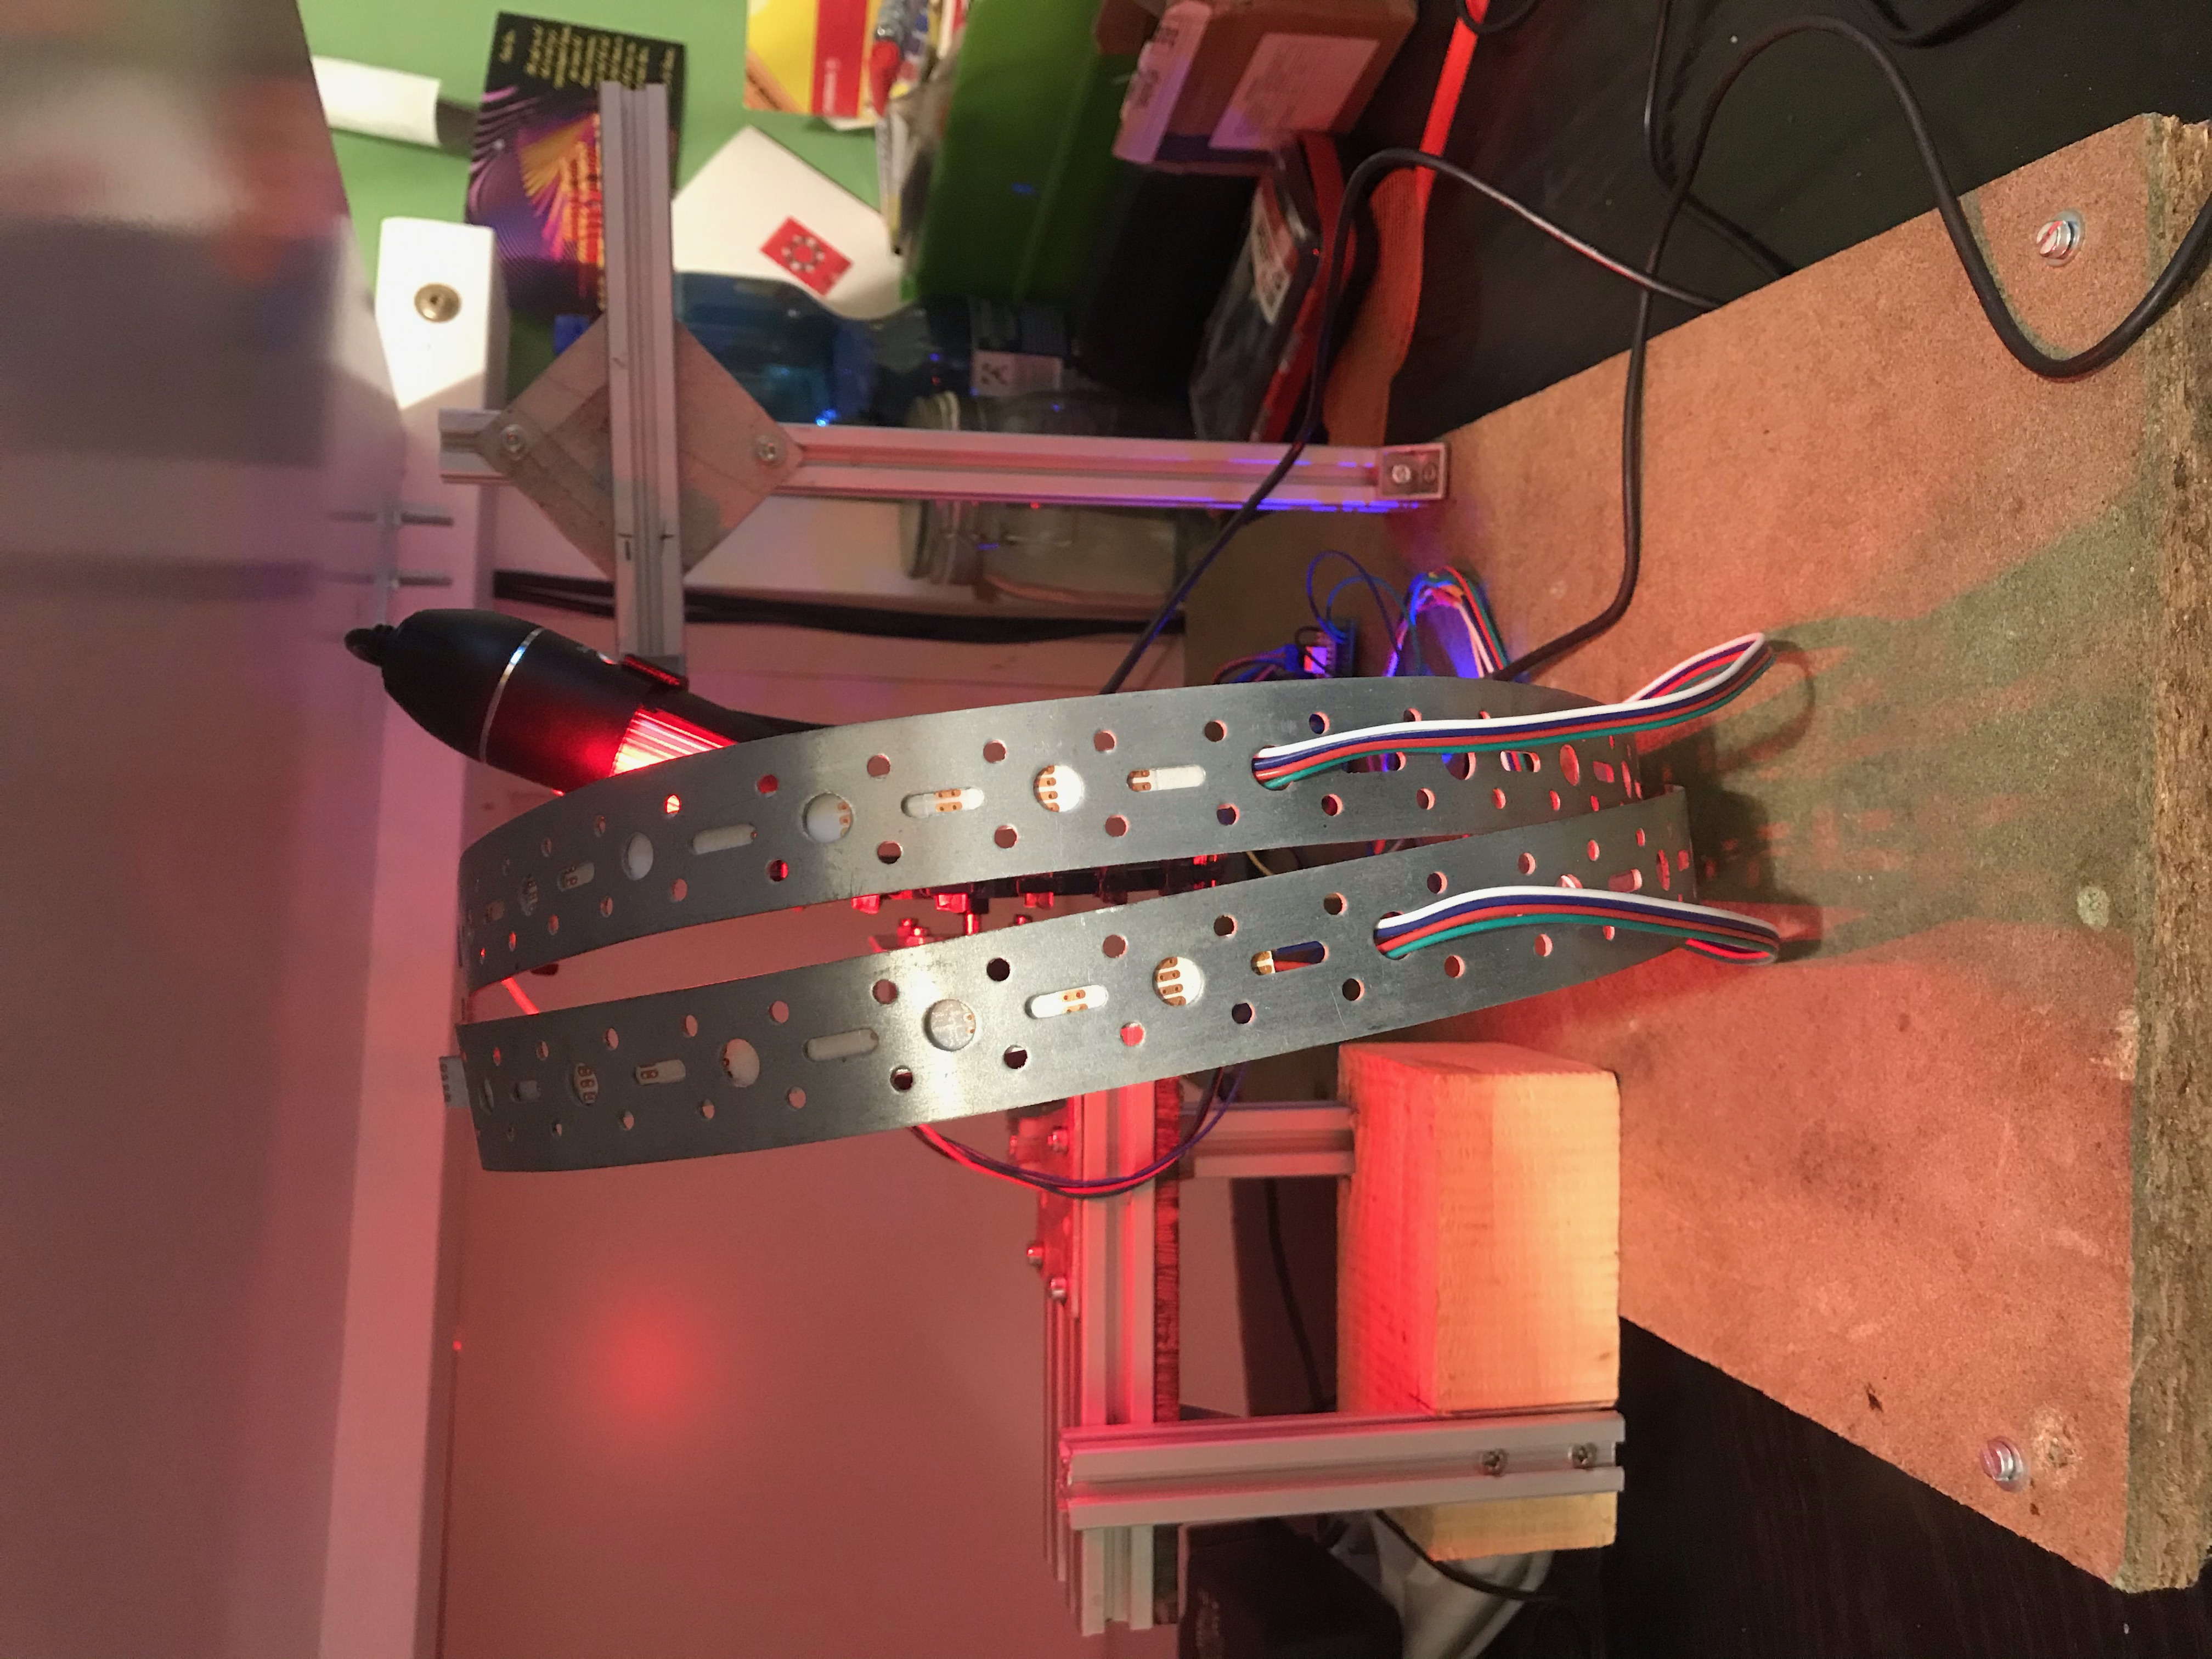
\includegraphics[width=4.166667in, keepaspectratio=true, angle=270]{./fig/Vision/Dataset/automated_datasets/2_created_datasets/2_Spaghetti_dataset/IMG_9295.jpeg}



The camera angle is kept the same a little to the top and very close to the inserts as seen on Figure \ref{fig:impl:sd:setup:top}

\begin{figure}[hbtp]
\centering
	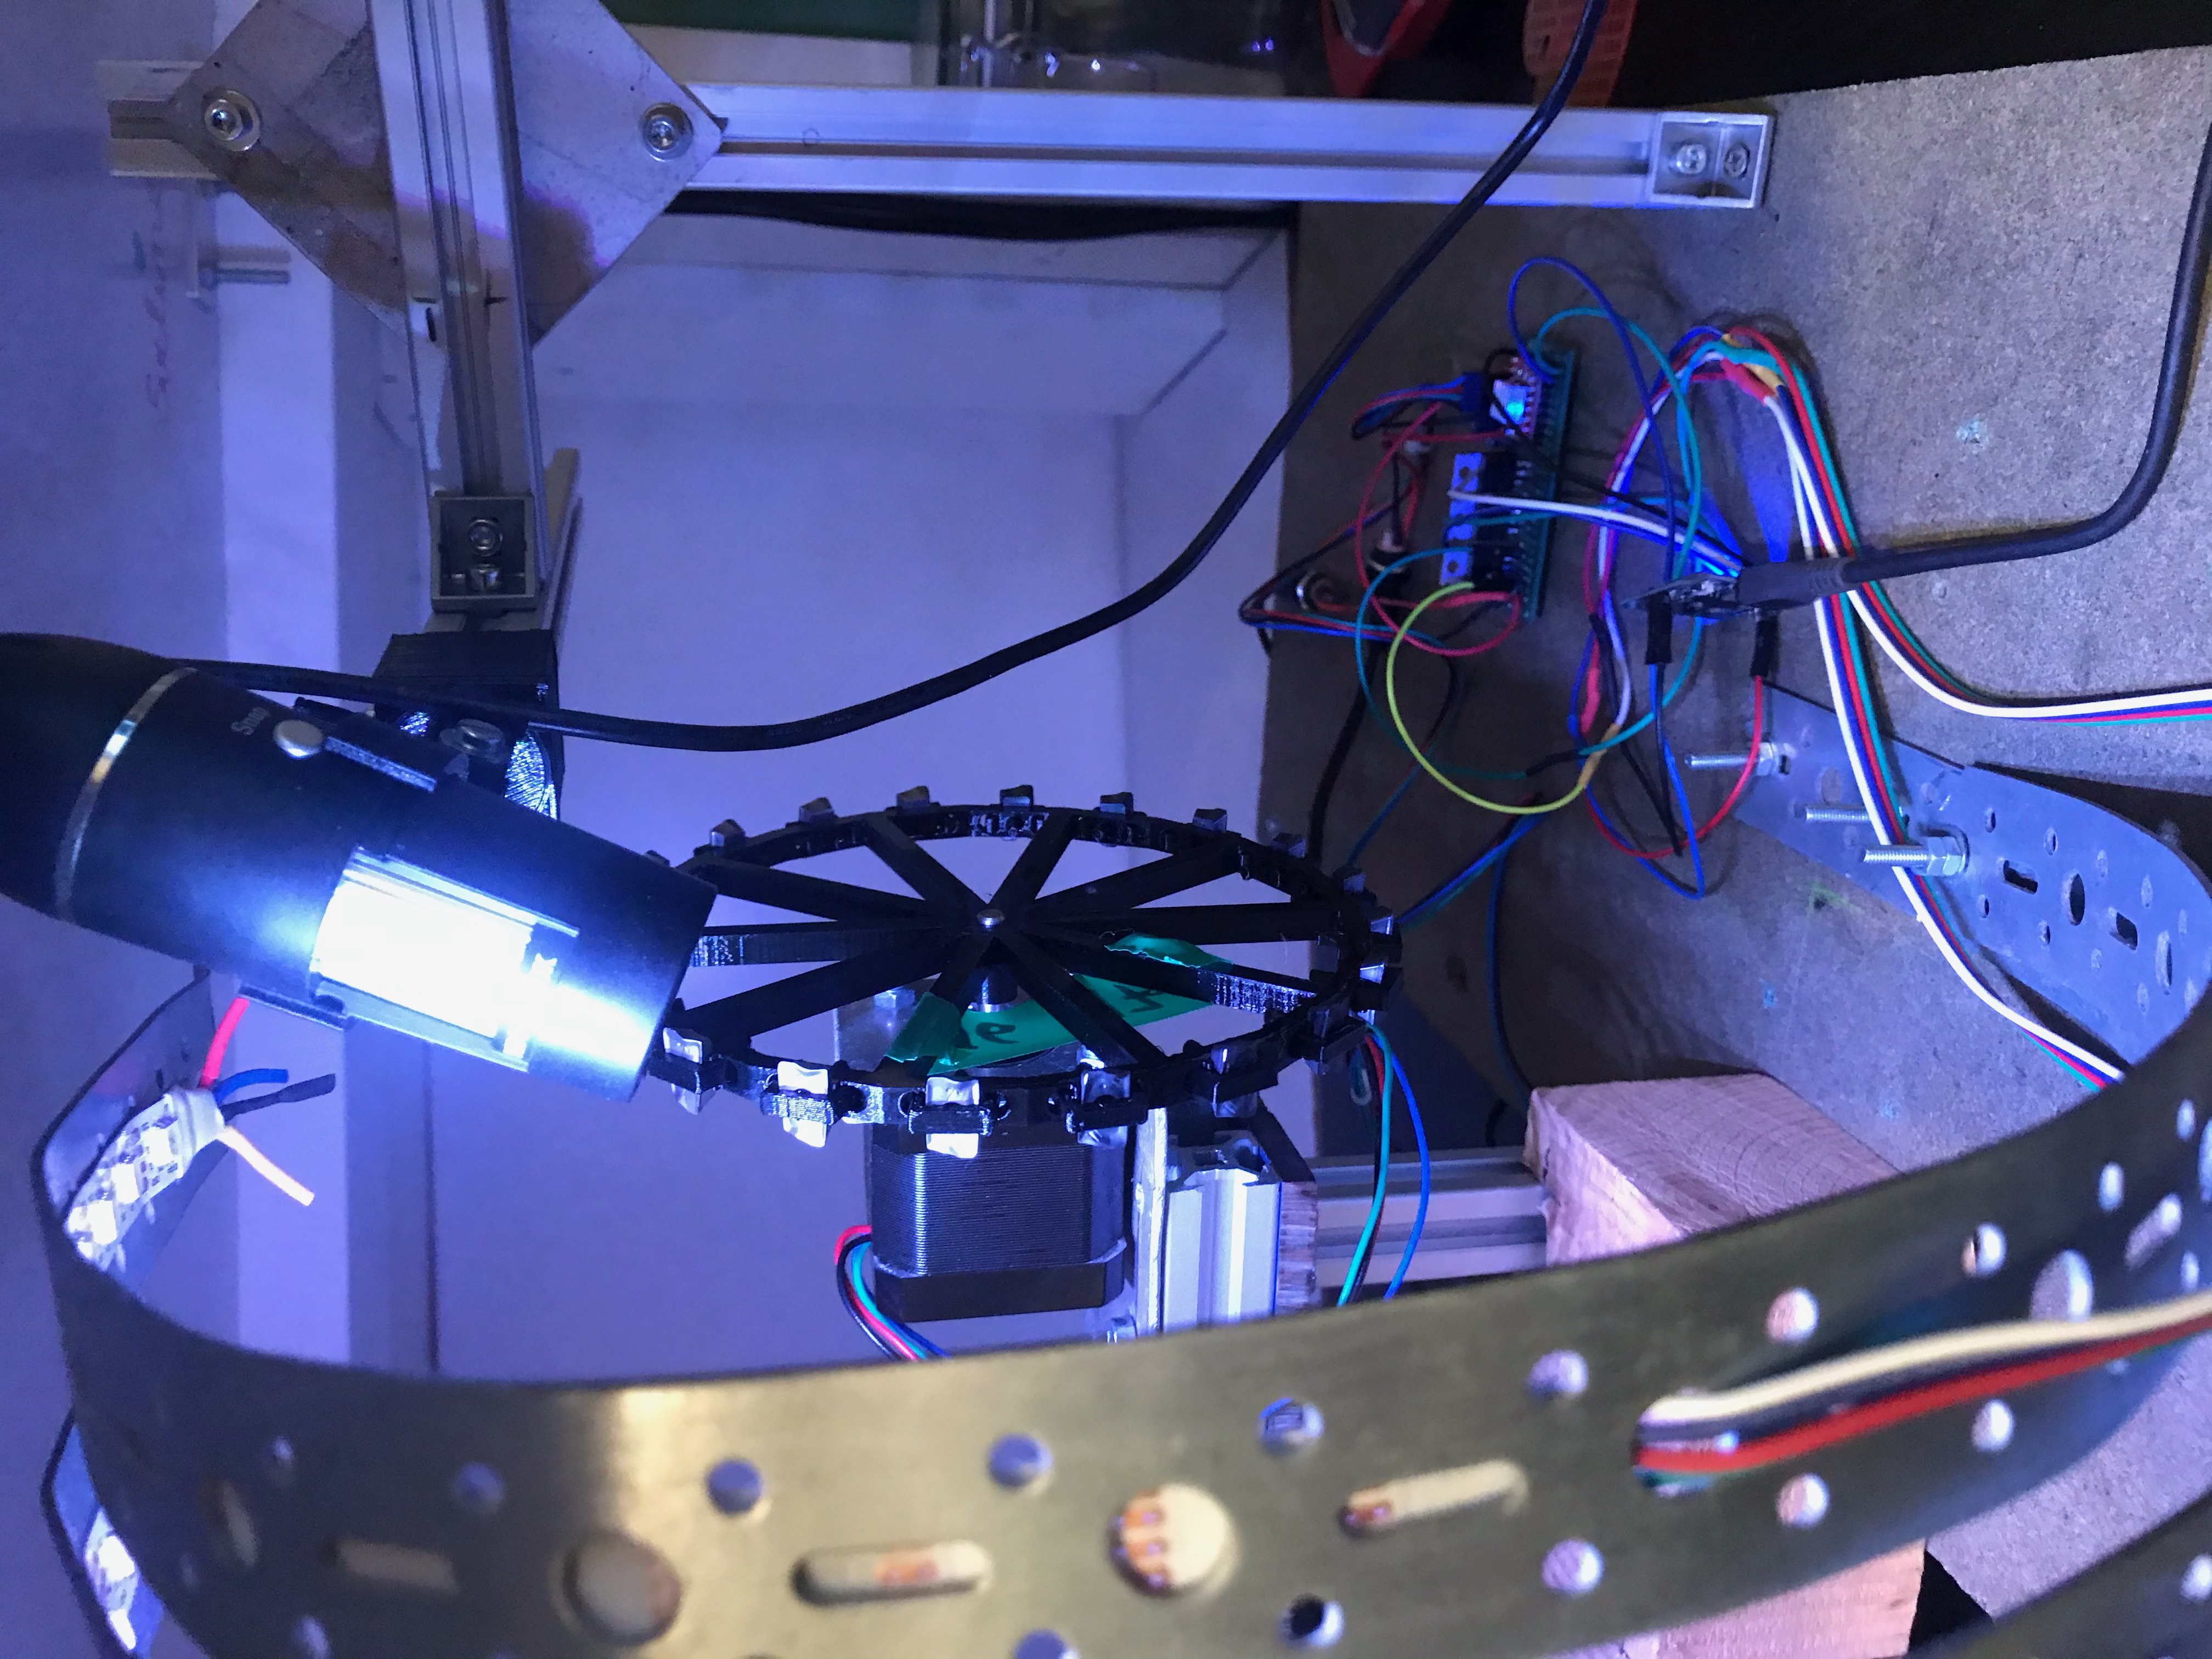
\includegraphics[width=4.166667in, keepaspectratio=true,angle=270]{./fig/Vision/Dataset/automated_datasets/2_created_datasets/2_Spaghetti_dataset/IMG_9296.jpeg}
	\caption{Test setup camera angle more to top.}
	\label{fig:impl:sd:setup:top}
\end{figure}



Through the whole dataset the direct light coming from other sources eg. the light of the room was blocked to have full control of the lighting conditions.



\subsection{Results}

Underneath are some pictures of good examples in the dataset.



Underneath are two pictures of batch 3 insert 6. These where lid with red light on the left and white light on the right. Here is a nice wear shown and lighted. However if we zoom in to the picture the top part of the wear is not lighted that well. We can also see a white piece of the insert holder on the image which is providing som extra difficulties. The discussion of these difficulties will be bespoken in vision algorithm.

\begin{figure}[hbtp]
	\centering
	\begin{subfigure}{0.49\textwidth}
		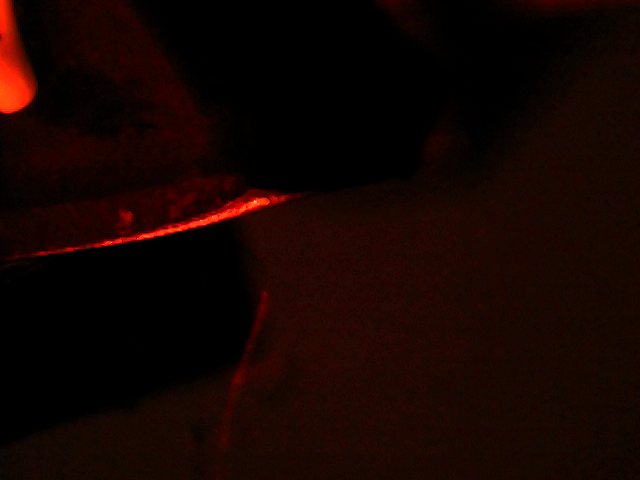
\includegraphics[width=3.125000in, keepaspectratio=true]{./fig/Vision/Dataset/automated_datasets/2_created_datasets/2_Spaghetti_dataset/b_003_p_006_l_006-011_red_nb.png}
		\caption{Red light}
	\end{subfigure}
	\hspace*{\fill}
	\begin{subfigure}{0.49\textwidth}
		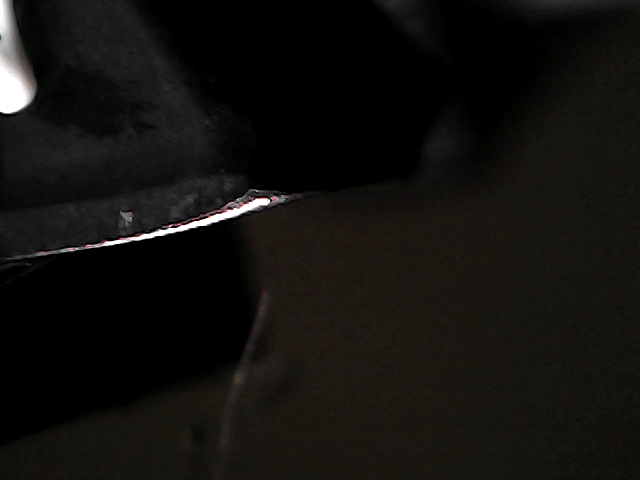
\includegraphics[width=3.125000in, keepaspectratio=true]{./fig/Vision/Dataset/automated_datasets/2_created_datasets/2_Spaghetti_dataset/b_003_p_006_l_006-011_white_nb.png}
		\caption{White light}
	\end{subfigure}
	\caption{Example images for red and white light for spaghetti dataset.}
\end{figure}



Some pictures aren't sharp like the one shown next.

like batch 5 insert 5 withoud bullet.
\begin{figure}[hbtp]
	\centering
	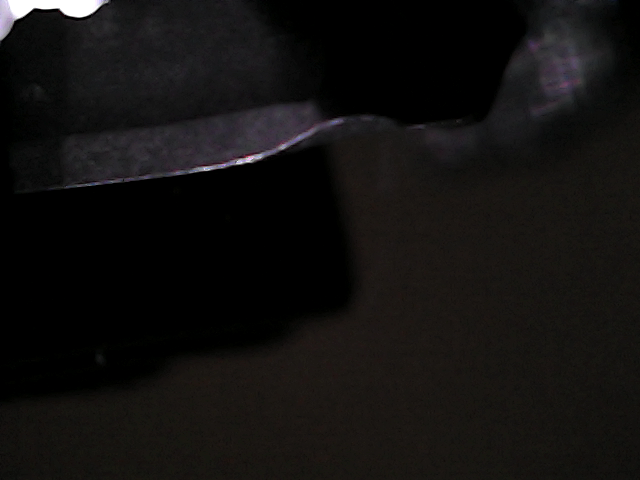
\includegraphics[width=3.125000in, keepaspectratio=true]{./fig/Vision/Dataset/automated_datasets/2_created_datasets/2_Spaghetti_dataset/b_005_p_005_l_006-011_white_nb.png}
	\caption{Unsharp image}
\end{figure}



\paragraph{Different insert types}

First type are the grey inserts with very visible wear. These are seen in batches 1 to 5 consistently. This type will be called grey inserts.

Than there are other inserts in batch 11 which are also grey but have a different shape on the cutting part. These will be called rounded grey inserts.

In batch 12 and 13 there are the same shape of inserts but with a black coating which results in way darker pictures as seen here on batch 13 insert 2 no bullet. These inserts are the rounded black inserts.

The next type are copper colored inserts with the rounded shape. Seen in batch 14 insert 5 no bullet.

Than we have inserts with a gold coating and hooked shape. For batch 15 insert 6 no bullet that gives the next picture:

\begin{figure}[hbtp]
	\centering
	\begin{subfigure}{0.49\textwidth}
		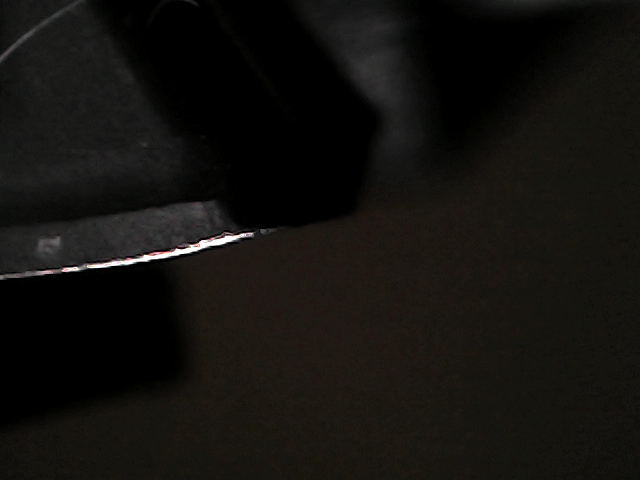
\includegraphics[width=3.125000in, keepaspectratio=true]{./fig/Vision/Dataset/automated_datasets/2_created_datasets/2_Spaghetti_dataset/gray_b_003_p_004_l_006-011_white_nb.png}
		\caption{Grey insert with very visible wear.}
	\end{subfigure}
	\hspace*{\fill}
	\begin{subfigure}{0.49\textwidth}
		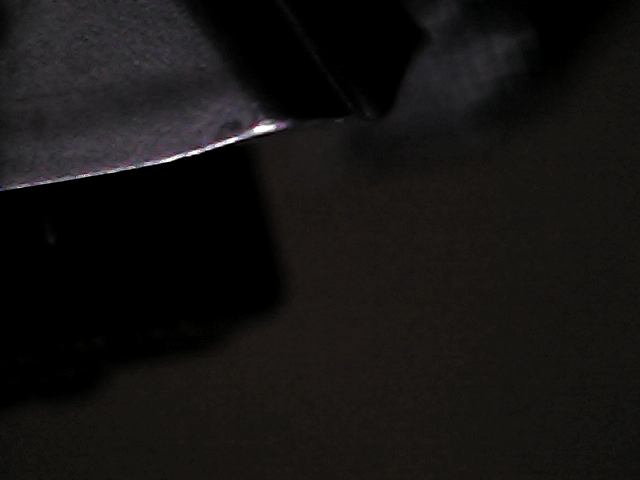
\includegraphics[width=3.125000in, keepaspectratio=true]{./fig/Vision/Dataset/automated_datasets/2_created_datasets/2_Spaghetti_dataset/rounded_grey_b_011_p_008_l_006-011_white_nb.png}
		\caption{Rounded grey insert.}
	\end{subfigure}
	\hspace*{\fill}
	\begin{subfigure}{0.49\textwidth}
		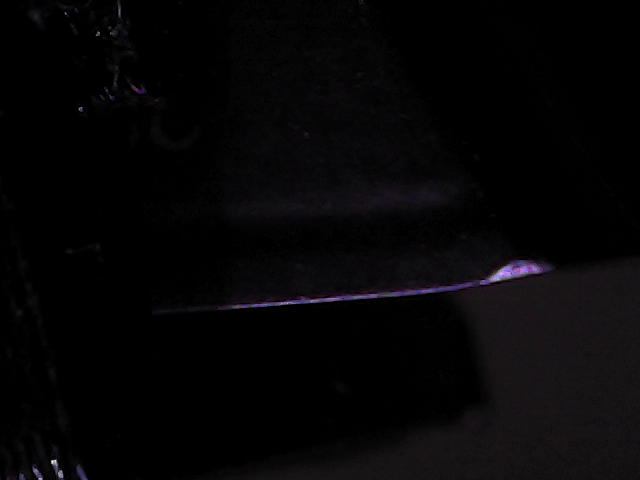
\includegraphics[width=3.125000in, keepaspectratio=true]{./fig/Vision/Dataset/automated_datasets/2_created_datasets/2_Spaghetti_dataset/rounded_black_b_013_p_002_l_006-011_white_nb.png}
		\caption{Rounded black insert.}
	\end{subfigure}
	\hspace*{\fill}
	\begin{subfigure}{0.49\textwidth}
		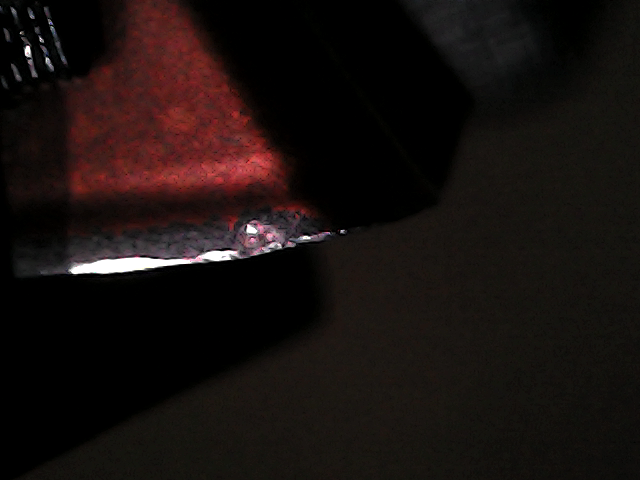
\includegraphics[width=3.125000in, keepaspectratio=true]{./fig/Vision/Dataset/automated_datasets/2_created_datasets/2_Spaghetti_dataset/rounded_copper_b_014_p_005_l_006-011_white_nb.png}
		\caption{Copper coloured insert.}
	\end{subfigure}
	\hspace*{\fill}
	\begin{subfigure}{0.49\textwidth}
		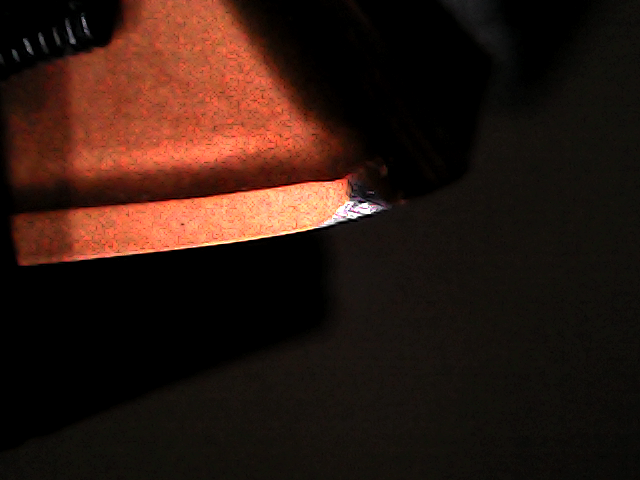
\includegraphics[width=3.125000in, keepaspectratio=true]{./fig/Vision/Dataset/automated_datasets/2_created_datasets/2_Spaghetti_dataset/rounded_gold_b_015_p_006_l_006-011_white_nb.png}
		\caption{Gold coloured insert.}
	\end{subfigure}
\end{figure}



\section{Google Colab}
\section{Test Camera Setup}

Created woensdag 04 november 2020



To test the camera setup, a binary classification model is made. This model will tell with a treshold of 150 (200 the real treshold but 150 to warn before tool is worn out) wether a tool is good to work with or must be removed from the machine. 

This model should be trainable with as less images as possible, preferably 20 because that is the amount of pictures taken in one batch.





\subsection{Resnet18}

First we will try to implement SDD-Resnet18 to classify the few images in good or bad. 



\subsection{nception v3}

Than we will implement SDD-inception v3 



These described models should perform rather good without any transfer learning. 

After the first tests these results can be compared with a transfer learning model.





\subsection{All Networks}

For this all networks test, some networks where tested and an algorithm is created to make it possible to add more networks along the way


		\section{All Networks}

Created woensdag 02 december 2020




		\section{All Networks 1}

Created woensdag 02 december 2020



All networks 1 can be found \href{https://colab.research.google.com/drive/1bWt0DgypiYoOOgnSGjlmSdDo7elvJnH4}{here.}



\subsection{Network architectures}

This model is used to test different model architectures namely:

\begin{itemize}
\item Resnet18
\item Alexnet
\item VGG11\_bn
\item Squeezenet
\item Densenet
\end{itemize}


inception v3 didn't seem to work



These models are all relatively small and should provide quite good results for a small dataset. 

More on why the models should work can be found here



\subsection{Dataset}



This algorithm had the input of images from the Second handmade dataset which was devided into 3 classes based on their measured wear value. 

\begin{tabular}{ |l|l|l| }
\hline
 class & min value (micron) & max value (micron) \tabularnewline
\hline
\hline
 good & 0 & 130 \tabularnewline
\hline
 medium & 130 & 230 \tabularnewline
\hline
 bad & 230 & infinity \tabularnewline
\hline
\end{tabular}










\subsection{Results}

Results of this notebook are available on wandb as \href{https://wandb.ai/dplars/pytorch-TWI_second_handmade?workspace=user-dplars}{pytorch-TWI\_second\_handmade}



Interesting results will be bespoken here;

Tests for different models: 

\begin{tabular}{ |l|l|l|l| }
\hline
 model name & test accuracy \% & validation accuracy\% & transfer learning \tabularnewline
\hline
\hline
 Alexnet & 100 & 90 & yes \tabularnewline
\hline
 VGG11\_bn & 89 & 85 & yes \tabularnewline
\hline
 Densenet & 89 & 85 & yes \tabularnewline
\hline
 Squeezenet & 89 & 85 & yes \tabularnewline
\hline
 Resnet18 & 89 & 90 & no \tabularnewline
\hline
\end{tabular}
										

An overview of the best runs for every model architecture. Since there are only nine test images; the test scores are set to a very high granularity. Further results of this test are to be found on wandb as \href{https://wandb.ai/dplars/pytorch-TWI_second_handmade/reports/Testing-on-first-handmade-dataset--VmlldzozNTE5NzM}{Testing on first handmade dataset}


		\section{All Networks 2}

Created vrijdag 04 december 2020



\subsection{Network architectures}

This model is used to test different model architectures namely:

\begin{itemize}
\item Resnet18
\item Alexnet
\item VGG11\_bn
\item Squeezenet
\item Densenet
\end{itemize}


inception v3 didn't seem to work



These models are all relatively small and should provide quite good results for a small dataset. 

More on why the models should work can be found here



\subsection{Dataset}



This algorithm had the input of images from the Second handmade dataset which was devided into 3 classes based on their measured wear value. 

\begin{tabular}{ |l|l|l| }
\hline
 class & min value (micron) & max value (micron) \tabularnewline
\hline
\hline
 good & 0 & 130 \tabularnewline
\hline
 medium & 130 & 230 \tabularnewline
\hline
 bad & 230 & infinity \tabularnewline
\hline
\end{tabular}










\subsection{Results}

Results of this notebook are available on wandb as \href{https://wandb.ai/dplars/pytorch-TWI_second_handmade?workspace=user-dplars}{pytorch-TWI\_second\_handmade}



Interesting results will be bespoken here;

Tests for different models: 

\begin{tabular}{ |l|l|l|l| }
\hline
 model name & test accuracy \% & validation accuracy\% & transfer learning \tabularnewline
\hline
\hline
 Alexnet & 100 & 100 & yes \tabularnewline
\hline
 Resnet18 & 100 & 95 & no \tabularnewline
\hline
 Densenet & 100 & 85 & yes \tabularnewline
\hline
 Squeezenet & 100 & 85 & yes \tabularnewline
\hline
 VGG11\_bn & 100 & 90 & no \tabularnewline
\hline
\end{tabular}
										

An overview of the best runs for every model architecture. Since there are only nine test images; the test scores are set to a very high granularity. Further results of this test are to be found on wandb as \href{https://wandb.ai/dplars/pytorch-TWI_second_handmade/reports/Testing-on-first-handmade-dataset--VmlldzozNTE5NzM}{Testing on first handmade dataset}





Trying to sweep over different parameter settings didn't work on my local computer; all runs failed or crashed


		\section{All Networks 3 Birthday}

Created vrijdag 04 december 2020



The code for this project is to be found here: \href{https://colab.research.google.com/drive/1_DKPtHi231TMalsj-uaBLytjcX2DuyV4#scrollTo=vmsTN_T4xoXP}{TSU\_AllNetworks\_3\_Birthday}


		\section{All Networks 4 Spaghetti}

Created vrijdag 04 december 2020



The code for this can be found in here: \href{https://colab.research.google.com/drive/1kKCU9pAsVRqNR-lX1p45Z7BLTxp76CMq}{TSU\_AllNetworks\_4\_spaghetti}





The report is noted in \href{https://wandb.ai/dplars/pytorch-TWI_spaghetti_sweep/reports/Spaghetti-sweep-with-TSU_AllNetworks_4_spaghetti--VmlldzozNTIxNjM}{Spaghetti sweep with TSU\_AllNetworks\_4\_spaghetti} This can be transformed into latex without further problems i hope.


		\section{All networks 4 spaghetti first 5 batches}

Created vrijdag 04 december 2020



Only the first five batches are analysed in this report to check if the dataset is as good as the dataset created by hand of these batches.

Also the difference is checked between the red and white leds.




		
		\section{Resnet18}

Created woensdag 18 november 2020



In this page we will describe the results and actions taken to get results out of Resnet18



this paper suggests that this is a good architecture for a quite like problem. where a low amount of data is used.

	\emph{SDD-CNN: Small data-driven convolution neural networks for subtle roller defect inspection}
	


\subsection{Creating first file}



\subsection{TSU\_Resnet18\_1}



failed to load data, did copy files into correct directories and created dataset class



\subsection{TSU\_Resnet18\_2}



Simpeler method to read in data and not be able to change a lot of things;

next time build dataset class self with the same model. 

After that the regression model would be easy



First result of the training.

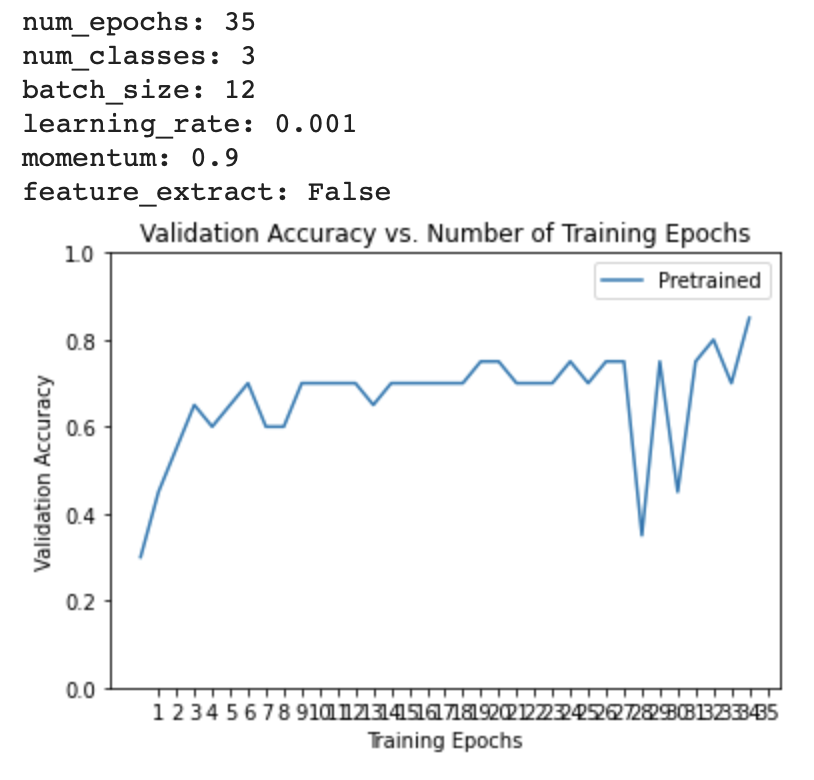
\includegraphics[height=4.166667in, keepaspectratio=true]{./fig/Vision/GoogleColab/Test_Camera_Setup/Resnet18/Screenshot 2020-11-18 at 22.58.45.png}

Tweede test met een aanpassing van de learning rate en een foto van de training set naar test set gebracht

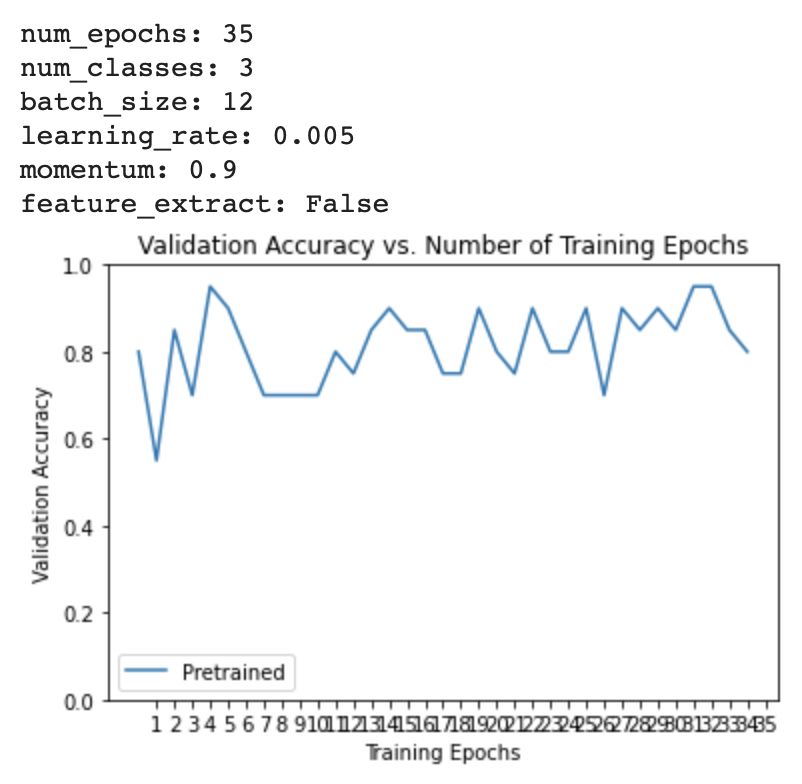
\includegraphics[height=4.166667in, keepaspectratio=true]{./fig/Vision/GoogleColab/Test_Camera_Setup/Resnet18/Screenshot 2020-11-18 at 23.13.23.png}



Next time create results file to get nice overview of all results


